\documentclass[linguex]{sp}
%\documentclass[11pt]{article}
%\usepackage[hmargin={.75in},vmargin={1.25in},foot={.6in}]{geometry}   
%\geometry{letterpaper}                   % ... or a4paper or a5paper or ... 
%\geometry{landscape}                % Activate for for rotated page geometry
%\usepackage[parfill]{parskip}    % Activate to begin paragraphs with an empty line rather than an indent
%\usepackage{graphicx,color}
%\usepackage{natbib}
\usepackage{booktabs}
%\usepackage{subfig}
%\usepackage{latexsym}
%\usepackage{amsmath}
%\usepackage{amssymb}
%\usepackage{amsthm}
%\usepackage{alltt}
%\usepackage{textcomp}
%\usepackage{url}
%\usepackage{epsfig}
%\usepackage{multicol}
%\usepackage{pstricks}
%\usepackage{tabularx}
%\usepackage{gb4e}
%\usepackage{qtree}
%\qtreecenterfalse
%\usepackage[normalem]{ulem}
%\usepackage{linguex}
%\usepackage{bbding}
%\usepackage{setspace}
%\usepackage[table]{xcolor}
%\usepackage{pifont} %ding
\usepackage{pst-node}
%\usepackage{bold-extra}

%\usepackage{natbib}

%\setcounter{secnumdepth}{4}

\newcommand{\txtp}{\textipa}
\renewcommand{\rm}{\textrm}
\newcommand{\sem}[1]{\mbox{$[\![$#1$]\!]$}}
\newcommand{\lam}{$\lambda$}
\newcommand{\lan}{$\langle$}
\newcommand{\ran}{$\rangle$}
\newcommand{\type}[1]{\ensuremath{\left \langle #1 \right \rangle }}
\newcommand{\defeq}{$\mathrel{\mathop:}=$ }
\renewcommand{\and}{$\wedge$ }
\renewcommand{\tt}{\texttt}
\newcommand{\op}{$\oplus$}


\newcommand{\bex}{\begin{exe}}
\newcommand{\eex}{\end{exe}}

%bullet points
\newcommand{\bit}{\begin{itemize}}
\newcommand{\eit}{\end{itemize}}

%numbering, non sequential
\newcommand{\ben}{\begin{enumerate}}
\newcommand{\een}{\end{enumerate}}

%\linespread{1.2}




% \pdf* commands provide metadata for the PDF output. ASCII characters only!
\pdfauthor{Gregory Scontras and Noah D. Goodman}
\pdftitle{Resolving uncertainty in plural predication}
\pdfkeywords{Full keyword list, separated, by, commas}

% Optional short title inside square brackets, for the running headers.
% If no short title is given, no title appears in the headers.
\title[Resolving uncertainty in plural predication]{Resolving uncertainty in plural predication \thanks{We thank people. XXX}}

% Optional short author inside square brackets, for the running headers.
% If no short author is given, no authors print in the headers.
\author[Scontras \& Goodman]{% As many authors as you like, each separated by \AND.
	\spauthor{Gregory Scontras \\ \institute{Stanford University}} \AND
	\spauthor{Noah D.~Goodman \\ \institute{Stanford University}}
}





\begin{document}

\maketitle

\begin{abstract}
	Predicates like \textit{heavy} or \textit{expensive} admit ambiguities in interpretation when used to ascribe properties to sets of objects. \textit{The boxes are heavy} can mean either that each member of some salient set of boxes is heavy, or that, taken together, the set of boxes collectively counts as heavy (even if no individual member is). Not all predicates are so permissive in their interpretations: \textit{The boxes are big} most likely communicates that each box is big --- the collective interpretation whereby speakers communicate directly about total set size is often hard to come by. We explain this divergence by showing that the probability of an interpretation depends crucially on potential variability in the property being communicated. Collective weight is a stable property of sets: Stacking boxes on top of each other or lining them up side by side, the total weight of those boxes remains the same, and corresponds to the sum of the weights of each box. The collective interpretation that eludes predicates like \textit{big} or \textit{wide} or \textit{long} or \textit{tall} depends crucially on the way that a set of objects is arranged physically (e.g., stacked one on top of the other, lined up side by side, etc.). The collective size of a set will therefore change depending on the physical arrangement of the members of that set. Manipulating variability in interpretation by decreasing noise in physical arrangement makes a collective interpretation more likely: If sets of boxes regularly come stacked on top of each other, \textit{The boxes are big} is more likely to communicate that the total size of some set of boxes is large. These facts support a general model of rational communication under which the resolution of ambiguities is sensitive to the amount of variability in possible interpretations: A more variable interpretation is potentially less informative because it requires more coordination between speakers and listeners. The interpretation is therefore less likely.
\end{abstract}

\begin{keywords}
	XXX (special formatting is fine)
\end{keywords}

\newpage

\tableofcontents

\newpage


\section{Introduction}

Predicates like \textit{heavy} or \textit{expensive} admit both distributive and collective interpretations: \textit{The boxes are heavy} can mean either that each member of some salient set of boxes is heavy (distributive), or that taken together the whole set counts as heavy (collective; \citealp{scha1984}). Crucially, the set of boxes may count as collectively heavy even when each individual box counts as light. In such a scenario, distributive and collective interpretations pull apart, suggesting a genuine ambiguity in plural predication.

Not all predicates are so permissive in their interpretations. Since \citet[140]{quine1960}, linguists have assumed that certain predicates lack collective interpretations: \textit{The boxes are big} is said to communicate only about individual box size; the collective interpretation whereby speakers communicate about total set size is claimed to be absent (or at least extremely hard to come by). Other size and shape predicates are said to behave similarly (e.g., \emph{long}, \emph{round}); \cite{schwarzschild2011} terms them ``stubbornly distributive,'' signaling the lack of collective interpretations. \citet{zhang2013} labels this class of predicates ``delimitable,'' highlighting their usage to describe physical extents. \cite{syrett2015} finds evidence of stubborn distributivity in children as young as 3 years of age.

Understanding why (and whether) stubbornly distributive predicates like \emph{big} differ from complaisantly collective predicates like \emph{heavy} requires understanding the more basic issue of the role of context in plural predication. As we will see, context plays a central role in the choice between distributive and collective interpretations. Determining how casts the distributive/collective distinction in a new light, while illuminating the semantics of plural predication and the pragmatic mechanisms of ambiguity resolution. 

To address the question of how much plural predication depends on context, and in what way, we establish a way of studying plural predication experimentally. In Expt.~1, we introduce and validate a new paraphrase methodology, which probes possible interpretations with unambiguous paraphrases. The results of Expt.~1 demonstrate a difference between \emph{big} and \emph{heavy}, as expected, but show that the predicate \emph{tall} patterns with \emph{heavy} in its ability to yield collective interpretations, at least in our experimental setting. We take these findings as evidence that stubborn distributivity cannot be reduced simply to predicating properties of physical extent.

We then explore the idea that contextual predictability of the relevant collective property is a critical factor in determining which reading is used. Expt.~2 uses the paraphrase endorsement methodology to show that less variable contexts make collective interpretations more acceptable for all of the predicates tested. Finally, we discuss the role of contextual predictability and speaker knowledge under a pragmatic account of ambiguity resolution in plural predication, using a lifted-variable variant of a Bayesian Rational Speech-Act model to formalize the process \citep{frankgoodman2012,lassitergoodman2013}.

But first, a primer on the semantics of plural predication writ broad, and then some background on gradable predicates and stubborn distributivity specifically.

\subsection{Representations of plurality}

The foundational work in the semantics of plurality is \cite{link1983}; he adopts a mereological account of the logical structure of plurality. \citeauthor{link1983} bases many of his claims on observations concerning the behavior of nominal conjunctions in English --- these, he assumes, name pluralities; the sentences in \Next[a] together entail the sentence in \Next[b]. If each individual is a man, then taken together they are men.

\ex. \label{cumulative}\a. Alan is a man. Bill is a man. Charlie is a man.
\b. Alan, Bill, and Charlie are men.

To understand the \textsc{cumulative} inference in \Last, \citeauthor{link1983} makes some assumptions concerning the domain of individuals, together with the formal mechanism of predication (i.e., ascribing properties to individuals): set inclusion \citep[cf.][]{montague1973}.

First, the domain of individuals, D$_{e}$, consists of atomic individuals --- objects in the domain without other objects as (proper) individual parts. This set includes individuals like Alan, Bill, Charlie, the book on your shelf, an apple, and so on. Predicates are modeled as sets of individuals --- those individuals that hold the property named by the predicate. The denotation of a singular nominal predicate like (\emph{is a}) \emph{man} is a subset of this atomic domain.

\ex. \label{theboys} Let \sem{Alan} = \texttt{a}, \sem{Bill} = \texttt{b}, and \sem{Charlie} = \texttt{c}; assume no other men. Then,\\
 \sem{(is a) man} = \{\texttt{a}, \texttt{b}, \texttt{c}\}

Singular \emph{man} contains all and only those members of the atomic domain that hold the property of being a man --- it contains the men in the domain. In \Last, where we assume three men, the set denoted by singular \emph{man} contains just Alan, Bill, and Charlie, or the individuals \tt{a}, \tt{b}, and \tt{c}.

Given the model sketched in \Last, and assuming predication gets modeled as set inclusion, the derivation in \Next results as we say of the sentence \emph{Alan is a man} that it is true: Alan is a man just in case he is a member of the set of singular men; Alan is in fact a member of the set of singular men, so he is a man.

\ex. \sem{Alan is a man} = 1 iff\\
\sem{man}(\sem{Alan}) = 1, i.e., iff\\
\texttt{a} $\in$ \{\texttt{a}, \texttt{b}, \texttt{c}\}

To achieve a general theory of predication, \citeauthor{link1983} must say how set inclusion transpires with plural predicates like \emph{men}; but first, \citeauthor{link1983} must take a stance on plural reference more broadly: (plural) individuals are modeled as mereological sums, points on mereological lattices that track part-whole relations. Simply put, a plurality is a sum of its parts: the plural individual named by \emph{Alan, Bill, and Charlie} is the summation of the singular individuals \tt{a}, \tt{b}, and \tt{c}. 

For \citeauthor{link1983}, pluralities are formed via the \textsc{individual sum} operator $\oplus$, which spells out in English as (some variants of) the conjunction \emph{and}.

\ex. For any two individuals \texttt{x}, \texttt{y}, their sum (i.e., the individual named by \emph{x and y}) is the smallest plural individual that has \texttt{x} and \texttt{y} as parts: \texttt{x}$\oplus$\texttt{y}

If there are three boys, as in \ref{theboys}, then \emph{the boys} names the same plural individual as \emph{Alan and Bill and Charlie}, namely \texttt{a}$\oplus$\texttt{b}$\oplus$\texttt{c}. The spatial, structural, and functional arrangement of this sum is left unspecified. It merely represents the collection, however arranged, of the three individuals.

Now, (semantically) plural nominal predicates (e.g., \emph{men}) contain pluralities in their extensions; to build a plural predicate from singular ones, \citeauthor{link1983} introduces the `star'-operator, *, which takes a predicate \texttt{P} and generates all of the individual sums of members of the extension of the basic, `un-starred' predicate. Roughly speaking, a plural predicate, *\texttt{P}, is a collection of all of the possible subsets of the singular predicate \texttt{P} (less the empty set \O).

\ex. \sem{*\texttt{P}} \defeq \{\texttt{x} $\in$ D$_{e}$: $\exists$\texttt{X} $\subseteq$ \sem{\texttt{P}}[\texttt{X} $\neq$ \O\ \and \texttt{x} = \texttt{S}(\texttt{X})]\}\\
where \texttt{S}(\texttt{X}) is the supremum, or maximal element of \texttt{X}

We can now model the denotation of English \emph{man} and \emph{men} using the sets in \Next; \emph{man} corresponds to the singular property of being a man, while \emph{men} corresponds to the closure of that property under sum-formation via the *-operator.\footnote{The present discussion collapses over the distinction between semantic and morphological plurality. See \cite{scontras2013salt,scontras2013sub,scontras2014diss} for fuller discussion of this distinction.} \emph{Men} thus denotes the set of all men and their possible combinations.

\ex. \texttt{P} = \texttt{man}\\
\sem{\texttt{P}} = \{\texttt{a}, \texttt{b}, \texttt{c}\}\\
\sem{*\texttt{P}} = \{\texttt{a}, \texttt{b}, \texttt{c}, \texttt{a}$\oplus$\texttt{b}, \texttt{a}$\oplus$\texttt{c}, \texttt{b}$\oplus$\texttt{c}, \texttt{a}$\oplus$\texttt{b}$\oplus$\texttt{c}\}

The semilattice in Fig.\ \ref{semilattice} conveys similar information, while explicitly tracking the part-whole relations among the individuals.
Each node $\bullet$ in Fig.\ \ref{semilattice} represents an individual in the domain, and the lines connecting the nodes track part-hood. For example, Alan and Bill are each individual parts of the plural individual named by \emph{Alan and Bill}, which itself is a part of the plural individual named by \emph{Alan, Bill, and Charlie}. Together, they are men, which means that each is a man.

\begin{figure}[t]
%\psset{rowsep=20pt,colsep=50pt,nodesep=4pt} 
\centering
\psset{rowsep=-2pt,colsep=10pt,nodesep=2pt} 
\hspace{80pt}\begin{psmatrix}
& \texttt{a}$\oplus$\texttt{b}$\oplus$\texttt{c} & \\
& \rnode{abc}{$\bullet$}\\
& & & & $\Leftarrow$ \textbf{Sums}\\
\rnode[t]{ab}{\texttt{a}$\oplus$\texttt{b}} & \rnode[t]{ac}{\texttt{a}$\oplus$\texttt{c}} & \rnode[t]{bc}{\texttt{b}$\oplus$\texttt{c}}\\
\rnode{ab2}{$\bullet$} & \rnode{ac2}{$\bullet$} & \rnode{bc2}{$\bullet$}\\
\\
\rnode{a}{$\bullet$} & \rnode{b}{$\bullet$} & \rnode{c}{$\bullet$} & & \ \ $\Leftarrow$ \textbf{Atoms}\\
\texttt{a} & \texttt{b} & \texttt{c}
\ncline{abc}{ab} \ncline{abc}{ac} \ncline{abc}{bc}
\ncline{ab2}{a} \ncline{ab2}{b}
\ncline{ac2}{a} \ncline{ac2}{c}
\ncline{bc2}{b} \ncline{bc2}{c}
\end{psmatrix}
\caption{The denotation of semantically plural \emph{men}, a complete atomic join semilattice}\label{semilattice}
\end{figure}

\noindent 

The mereological representation of individuals in terms of individual part-hood introduces a natural `part-of' ordering on the domain, $\leq_{i}$, which \citeauthor{link1983} represents in the object language using the predicate $\Pi$ `individual part of'; the bidirectional in \Next holds: if \tt{a} is an individual part of the individual \tt{b}, then the plural individual \tt{a}\op\tt{b} is identical to \tt{b}.

\ex. \tt{a}$\Pi$\tt{b}\ \ $\leftrightarrow$\ \ \tt{a}\op\tt{b} = \tt{b}

In Fig.\ \ref{semilattice}, the individual part relation $\Pi$ gets represented by the line segments connecting nodes. Pluralities, or `sums,' are those individuals which have other individuals in the domain as proper parts; atoms have no proper parts.

\subsection{Varieties of plural predication}

Given that plural predicates are constructed from singular ones via sum-formation, we may model the cumulative inference in \ref{cumulative} (repeated in \Next): if each of Alan, Bill, and Charlie are in the extension of the predicate \emph{man}, then their sum is necessarily in the extension of the semantically plural predicate \emph{men}; \emph{men} is the closure of \emph{man} under sum-formation, so if \tt{a}, \tt{b}, and \tt{c} are in the extension of \emph{man}, their sum \tt{a}\op\tt{b}\op\tt{c} must be in the extension of \emph{men}.

The distributive reading of \Next[b] follows from this semantics of plurality and predication, not any implicit quantification over the members of the subject. In other words, we need no  distributive operator (e.g., a silent \emph{each}) in the logical form of \Next[b] to derive \Next[a] as an entailment.

\ex. \a. Alan is a man. Bill is a man. Charlie is a man.
\b. Alan, Bill, and Charlie are men.

For Alan, Bill, and Charlie to be men, then \tt{a}\op\tt{b}\op\tt{c} --- the sum named by \emph{Alan, Bill, and Charlie} --- must be in the extension of the predicate named by \emph{men}. By assuming that \emph{men} corresponds to the closure of the singular predicate \emph{man}, it follows that each of Alan, Bill, and Charlie is a man whenever we say of Alan, Bill, and Charlie that they are men.

Here is where terminology begins to get confusing: For \citeauthor{link1983}, predicates may be inherently distributive; these are singular-seeking predicates like \emph{die} or \emph{see} or \emph{have blue eyes}; also, \emph{man}. These predicates entail a distributive reading whenever they are used.
Distributive predicates are those that contain only atoms in their basic (i.e., un-starred) denotations; to pluralize a distributive predicate --- so that it may apply to a plural argument via set inclusion --- we must close the predicate under sum formation via *, which ensures that for any plurality in the denotation of the plural predicate, each of its members is in the denotation of the singular predicate. Because plural predicates are formed via sum formation from singular predicates, and assuming distributive predicates contain only atoms in their singular denotations, then for a plurality to be in the denotation of a plural distributive predicate, each member of that plurality must be in the denotation of the singular predicate, as in \Next. Thus, it necessarily follows that if a plurality of individuals are men, each is a man.\footnote{The function \textsc{atom}(x) evaluates whether an individual is an atom in the domain; that is, whether it has any proper parts that are also in the domain.}

\ex. \a. \textsc{dist}(\texttt{P}) = 1 iff\\
$\forall$\texttt{x}[\texttt{P}(\texttt{x}) $\rightarrow$ \textsc{atom}(x)]
\b. For any \texttt{P}, \texttt{X}, if \textsc{dist}(\texttt{P}) and *\texttt{P}(\texttt{X}), then
$\forall$\texttt{x}$\Pi$\texttt{X}[\texttt{P}(\texttt{x})]


But not all predicates need be distributive, at least according to \citeauthor{link1983}. To illustrate this fact, he reproduces the following exchange between the German newspaper \emph{Frankfurter Allgemeine Zeitung} (FAZ) and the editor of \emph{Der Speigel}, Rudolf Augstein (RA): 

\ex. FAZ: ``Which property do you appreciate most with your friends?''\\
RA: ``That they are few.''

Being few is not a property any one of RA's friends holds. In fact, it makes no sense to say of an individual that he or she is few. Rather, the friends \textsc{collectively} hold this property. \citeauthor{link1983} models this fact by assuming that the predicate \emph{be few} contains in its basic, un-starred denotation pluralities of individuals. Suppose RA's friends are Alan, Bill, and Charlie, and that numbering three counts as being few.

\ex. \tt{P} = \tt{be-few}\\
\sem{\tt{P}} = \{\tt{a}\op\tt{b}\op\tt{c}, \ldots\}\\
\sem{*\tt{P}} = \{\tt{a}\op\tt{b}\op\tt{c}, \ldots\}

The collective interpretation of RA's response in \LLast follows from the fact that the (un-starred) predicate applies directly to pluralities; in fact, the predicate may apply \emph{only} to pluralities --- it is a so-called `plurality-seeking' predicate like \emph{gather} or \emph{meet} \citep{schwarzschild1994}. In opposition to \citeauthor{link1983}'s distributive, or singular-seeking predicates, plurality-seeking predicates \emph{must not} contain atoms in their basic denotations. (\citeauthor{link1983} calls these plurality-seeking predicates `collective,' yet another source of terminological confusion.)

According to the liturgy, distributive, singular-seeking predicates and collective, plurality-seeking predicates self-sort on conceptual grounds: Being a man is a property that necessarily applies to individuals, while being few or gathering together are properties that cannot apply to individuals. Note, however, that even necessarily collective predicates like \emph{be few} or \emph{gather} may apply to singular noun phrases that transparently refer to pluralities of individuals, as in \Next. For now we leave aside issues surrounding collective nouns like \emph{group} or \emph{committee}. %Note, however, that if the distributive/collective divide bottoms out in  a prohibition on or requirement for singular individuals in the basic denotation of predicates, then our stance on the representation of these collective nouns must be compatible with such an approach.

\ex. The committee gathered in advance of the summit.\\
The group was too few to be taken seriously.\\
The army surrounded the castle. (cf. \emph{The soldier surrounded the castle})

%MASS NOUNS

For present purposes, the interesting cases are those predicates that are neither inherently distributive, applying only to atoms, nor inherently collective, applying only to sums; on many approaches, these mixed predicates contain both atoms and sums in their basic denotations. \citeauthor{link1983} gives the example \emph{build a raft}. Suppose Alan built a raft of his own, and Bill and Charlie built a raft together.

\ex. \tt{P} = \tt{build-raft}\\
\sem{\tt{P}} = \{\tt{a}, \tt{b}\op\tt{c}\}\\
\sem{*\tt{P}} = \{\tt{a}, \tt{b}\op\tt{c}, \tt{a}\op\tt{b}\op\tt{c}\}

With mixed predicates, the resulting interpretation is ambiguous; we may force either a distributive or a collective interpretation by adding words like \emph{each} or \emph{together}, respectively (a claim that we explore experimentally in Expt.~1 below). But without overt linguistic or contextual cues, the meaning of the bare predicate is underdetermined: \Next could mean either distributive \Next[a] or collective \Next[b].


\ex. Bill and Charlie built a raft.
\a. Bill and Charlie each built a raft. \hfill \textsc{distributive}
\b. Bill and Charlie together built a raft. \hfill \textsc{collective}


%\textcolor{red}{NOTE:}
%
%I am curious to know whether there are default preferences for mixed predicates in the unmarked case; to my ear, \Next defaults of a collective interpretation. \cite{link1998} claims that distributive predication is marked relative to collective predication cross-linguistically (with words like \emph{each}, etc.), which ought to predict a default collective interpretation for mixed predicates in the unmarked case. 
%
%\ex. Bill and Charlie built a raft.
%
%However, even if a collective reading is preferred for the unmarked mixed predicate in \Last, this preference likely stems from the singular object \emph{a raft}: to get a distributive reading for \Last, a listener would have to interpret \emph{a raft} as referring to more than one object, something they are loathe to do \citep[cf.\ the \emph{Single Reference Principle} of][]{kurtzmanmacdonald1993}.
%
%For what it's worth, with a bare plural object, my preference for a collective interpretation persists, but it is much weaker than with a singular object.
%
%\ex. Bill and Charlie built rafts yesterday.
%
%\textcolor{red}{END NOTE}

The distributive/collective distinction concerns the interpretation of argument positions; a single predicate with two arguments may have each argument interpreted in a different way. In \Next, we say of the plurality \emph{Jack and Jill} that together they carried each member of the plurality \emph{the piano and the bench}; in other words, we collectively ascribe the property of carrying to Jack and Jill, but distributively ascribe the property of being carried to the piano and the bench.

\ex. [Jack and Jill]$_{\textsc{coll.}}$ carried [the piano and the bench]$_{\textsc{dist.}}$ up the stairs.

Note also that a single noun phrase may receive different interpretations, varying by the predicates that take them as arguments. In \Next, we say of the suitcases A and B that each is light enough of to carry, but that together they belong to different passengers. It crucially does not follow from \Next that either of suitcases A or B independently belong to different passengers; the predicate is inherently collective, applying only to sums of individuals. It also does not follow that suitcases A and B are light enough to carry together; the predicate is mixed, and we know from the premises only that each suitcase --- but not their collection --- is light enough to carry.

\ex. \a.[] Suitcase A is light enough to carry.\\
Suitcase B is light enough to carry.\\
Suitcases A and B belong to different passengers.
 \b.[$\Rightarrow$] Suitcases A and B are light enough to carry and belong to different passengers.
 \citep[ex.(3)]{schwarzschild1994}

These facts suggest that plural meaning is a \emph{compositional}, and not a \emph{referential} phenomenon: a noun phrase does not have a collective or distributive referent, and neither does a verb have a collective or distributive denotation; rather, the composition of a noun phrase with a verb delivers distributive or collective interpretations. And as our study demonstrates, the meaning that results is sensitive to the context in which this composition occurs. To understand how, we must first understand sources of uncertainty endemic to this process of plural predication.

%We remarked briefly above on the underspecification of plural reference inherent to this semantics of plurality: individuals are summed together to create new, plural individuals, but the summation process remains intentionally vague. It remains to be shown, however, that our mental representations of these pluralities are as vague as their formal ones. For example, our representations of pluralities of real-world objects might track the physical arrangement of these objects, such that a set of boxes stacked one on top of the other and that same set of boxes lined up one next to the other count as different pluralities. In other words, we might view the summation operation \op\ as an umbrella term for the many ways of not merely collecting, but arranging sets of individuals.

The process of collective predication is inherently vague. Whereas distributive predication commits a speaker to relatively concrete statements about the state of the world --- if a plurality distributively holds some property, then each member holds that property --- collective predication admits much broader construals. We said that a plurality collectively holds a property when it belongs to the denotation of an `un-starred' predicate, but what (in the world) does this mean (in the world)? Take \emph{build a raft}: formally, a plurality of individuals \tt{a}\op\tt{b} collectively holds this property \tt{build-raft} whenever it is included in the denotation of the predicate, as in \Next.

\ex. \tt{P} = \tt{build-raft}\\
\sem{\tt{P}} = \{\tt{a}\op\tt{b}, \ldots\}

For the purposes of the semantics, the means by which a plurality gets included in the basic denotation of a predicate, that is, the means by which it collectively holds a property, remains a mystery. In the raft-building scenario, suppose we know that Alan and Bill together built a raft: a raft would not have resulted without the resources or efforts of both individuals. But do we know any more?

Rather than focusing our efforts on the nebulous interpretations of collective action statements, highlighted by predicates like \emph{build a raft}, we consider in detail a specific class of predicates with more concrete, (relatively) objective evaluation strategies: gradable adjectives like \emph{heavy} or \emph{big}.\footnote{XXX This is not to say that we know nothing about collective action statements. Something about Margaret Gilbert's Plural Subject Theory.} The measurement inherent to the semantics of these words delivers scalar interpretations that are amenable to quantitative study: for a collection of boxes to be heavy, big, tall, etc., they must have a certain weight, size, height. By examining intuitions about the use of these predicates, together with the predication context that delivers them, we stand to better understand the mechanism of plural predication: when collective interpretations are appropriate, what they communicate, and what mediates the choice between distributive and collective interpretations in the first place.


\section{Plurality and gradability}

Composing with a plurality, some gradable predicates either receive a \textsc{distributive} or a \textsc{collective} interpretation. Under a distributive reading, the relevant property gets ascribed to each member of the plural subject. Under a collective reading, we ascribe the property to the subject as a whole.

\ex. The boxes are heavy.
\a.[$\hookrightarrow$] the boxes each are heavy \hfill \textsc{distributive}
\z. or
\a.[$\hookrightarrow$] the boxes together are heavy \hfill \textsc{collective}

In this latter case, where we collectively ascribe a gradable property to a plurality, the resulting interpretation involves sum-based aggregation strategies: If a set of boxes together holds the property of being heavy, it follows that their total weight counts as heavy \citep{scha1984}.\footnote{For now we set aside the possibility of mean-based aggregation strategies, demonstrated for plural comparisons by \cite{scontrasetal2012}.} The reading becomes more transparent when we add a collective particle like \emph{together}. Crucially, a collective reading can be true when the distributive reading is false: many light boxes may together count as heavy. These two diverging interpretations suggest a semantics for the gradable predicate \emph{heavy} under which it applies both to singular objects and pluralities in its basic, un-starred form; it is a mixed predicate, like \emph{build a raft}. 

%Suppose we have four boxes: the first independently counts as heavy, while the latter three together do.
%
%\ex. \tt{P} = \tt{heavy}\\
%\sem{\tt{P}} = \{\tt{a}, \tt{b}\op\tt{c}\op{d}, \ldots\}\\
%\sem{*\tt{P}} = \{\tt{a}, \tt{b}\op\tt{c}\op{d}, \tt{a}\op\tt{b}\op\tt{c}\op\tt{d}, \ldots\}
%
%Here we face a  problem: With a monotonic predicate like \emph{heavy}, there is no difference in extension between the basic, un-starred predicate and its plural version, closed under sum formation. For any singular or plural individual in the denotation of the basic predicate, its combination with any other member of the basic predicate must also be in the denotation of the basic predicate. This result follows from the monotonicty of the named property: if something counts as heavy, then that thing plus another thing also counts as heavy. More worrisome is the explosion of the basic predicate denotation: whenever at least one object in the domain counts as heavy, it together with any other object in the domain must also count as heavy.
%
%Once we level the distinction between singular (un-starred) and plural (starred) predicates, collective inferences follow whenever there is a plural argument. Suppose a speaker utters the sentence in \Next; to verify this sentence, the starred predicate in \Next[a] must contain in its denotation the sum of boxes A, B, and C: \tt{a}\op\tt{b}\op\tt{c}. For the denotation in \Next[a] to result, either the basic, un-starred predicate must contain each box independently (i.e., each box counts as heavy), as in \Next[b], or the un-starred predicate must contain the plurality itself, as in \Next[c].\footnote{Another possibility would have intermediate combinations of the three boxes in the denotation of the un-starred predicate.} Importantly, it follows from the monotonicity of \emph{heavy} that if each box is in the denotation of the basic predicate, then their sum must be as well, as in \Next[b].
%
%\ex. Boxes A, B, and C are heavy.
%\a. \sem{*\tt{heavy}} = \{ \ldots, \tt{a}\op\tt{b}\op\tt{c}, \ldots\}
%\b. \sem{\tt{heavy}$_{1}$} = \{\tt{a}, \tt{b}, \tt{c}, \ldots, \tt{a}\op\tt{b}\op\tt{c}, \ldots\}
%\b. \sem{\tt{heavy}$_{2}$} = \{\tt{a}\op\tt{b}\op\tt{c}, \ldots\}
%
%These inferences arise independently of the logical structure that delivers them: If three boxes each count as heavy, then by the same standard those boxes taken together must also count as heavy. In other words, a collective interpretation must always be available when \emph{heavy} composes with a plurality.

The collective interpretation available to \emph{heavy} proves elusive for most other gradable predicates. A speaker is hard-pressed to use the sentence in \Next to say of the boxes that their total size is large.

\ex. The boxes are big.
\a.[$\hookrightarrow$] the boxes each are big \hfill \textsc{distributive}
\z. but not
\a.[$\hookrightarrow$] the boxes together are big \hfill \textsc{collective}

Size and shape adjectives, in other words, predicates of physical extent, resist collective interpretations. In his discussion of the contrast, \citet{quine1960} describes stubbornly distributive predicates like \emph{big} in \Last as ``not cumulative,'' drawing a parallel with the nominal domain: Just as a count noun like \emph{boxes} insistently ``divides its reference'' among individual boxes (in contrast to mass nouns like \emph{water} which are aggresively cumulative, referring to maximal salient quantities of water), so too do stubbornly distributive predicates divide their predication. \citeauthor{quine1960}'s characterization of the phenomenon prefigures the formal semantics that follows him. As we sketched above, collective predication arises when a property is ascribed directly to a plurality, rather than distributed among its members. Stubbornly distributive predicates behave as such because they cannot contain pluralities in their basic denotations \citep{schwarzschild2011,vazquezrojas2012,zhang2013}.\footnote{In his characterization of stubborn distributivity, Schwarzschild first assumes that gradable adjectives are predicates of events \citep[e.g.,][]{higginbothamschein1989}. Thus, \emph{heavy} predicates over \textsc{heavy} events, \emph{big} over \textsc{big} events, etc. For \citeauthor{schwarzschild2011}, stubbornly distributive predicates are those that require their events to have only single participants. The details are not directly relevant for our purposes; what is relevant is the lexical distinction \citeauthor{schwarzschild2011} and others make between stubbornly distributive and complaisantly collective predicates.}

\citet{schwarzschild2011} uses the failed correspondences in \Next illustrate one strategy in drawing out the failed collective reading for these gradable predicates: employing periphrastic paraphrases of the predicate. For example, to assert that the total size of some set of boxes exceeds a salient size cutoff, we may say that those boxes take up a lot of space. However, taking up a lot of space is not, strictly speaking, synonymous with having a large collective size; these paraphrases point to the missing collective reading, but only indirectly. Moreover, these paraphrases more explicitly name the collective property that would have been intended under a collective construal of the gradable predicate.\\

\begin{minipage}{.405\textwidth}
	\ex.
	The boxes are large.\\
	The phone calls were long.\\
	The papers are round.
	
\end{minipage}
\begin{minipage}{.05\textwidth}
	$\neq$
\end{minipage}
\begin{minipage}{.5\textwidth}
	The boxes take up a lot of space.\\
	The phone calls lasted a long time.\\
	The papers form a circle.
\end{minipage}\\[5pt]

Replacing the definite plural subject noun with a group/collective noun \citep[i.e., an atomizer;][]{scontras2014diss} is another way to make available the elusive collective reading. Intuitively, these collective nouns transform the plurality (e.g., the boxes) into a single individual (i.e., a pile), which readily composes with the gradable predicate. Crucially, these collective nouns are used the fix the arrangement of the named plurality, and as a result collective predication succeeds.\\

\begin{minipage}{.405\textwidth}
	\ex.
	The boxes are large.\\
	The phone calls were long.\\
	The papers are round.
	
\end{minipage}
\begin{minipage}{.05\textwidth}
	$\neq$
\end{minipage}
\begin{minipage}{.5\textwidth}
	The pile of boxes is large.\\
	The series of phone calls was long.\\
	The arrangement of papers is round.
\end{minipage}\\[5pt]

Descriptively, stubbornly distributive gradable predicates pattern with the singular-seeking distributive predicates we encountered above in that they resist taking pluralities as arguments, which precludes the collective predication modeled in \Next[a], but is perfectly compatible with distributing the property over members of the plurality, as in \Next[b].

\ex. \a. \sem{\tt{big}} = \{\tt{a}\op\tt{b}\op\tt{c}, \ldots\}
\b. \sem{\tt{big}} = \{\tt{a}, \tt{b}, \tt{c}, \ldots\}\\
\sem{*\tt{big}} = \{\tt{a}, \tt{b}, \tt{c}, \ldots, \tt{a}\op\tt{b}\op\tt{c}, \ldots\}

Supporting the idea that stubbornly distributive gradable predicates refuse all but singular individuals from their basic denotations, \cite{schwarzschild2011} observes that mass nouns, which do not refer (at any accessible level) to singularities, are often infelicitous as arguments to these predicates.

\ex. \# The $\left\{\begin{array}{l}\text{wine}\\ \text{snow}\\ \text{traffic}\end{array}\right\}$ is big.

\citeauthor{schwarzschild2011} notes that  the facts in \Last crucially do not lead to the conclusion that mass nouns refer to simple pluralities \citep[cf., e.g.,][]{chierchia1998mass}. If the denotation of a mass noun was simply a sum of individual or material parts, then we should in principle be permitted to distribute the relevant property over its (minimal) parts. Moreover, the less strongly-self-connected the substance named  \citep[in the sense of][]{grimm2012}, the more felicitous the combination of mass nouns with stubbornly distributive predicates; fake mass nouns are fine, as are atomic substances (\citeauthor{grimm2012}'s ``aggregates''). Only those mass nouns without accessible, stable minimal parts like \emph{water} or \emph{blood} are truly incompatible with these predicates.

\ex. \a. The furniture is big. \hfill \emph{fake mass noun}\\
The mail is square.
\b. The grass is long. \hfill \emph{aggregate}\\
The rice is round.

Refining the description of stubborn distributivity, these predicates presuppose the (at least conceptual) atomicity of their arguments: they must contain only stable atoms in their basic denotation. But stating that stubbornly distributive predicates do not contain in their basic, un-starred denotation sums of individuals (in line with distributive predicates like \emph{have blue eyes} or \emph{be a man}) serves merely to describe the phenomenon. Having blue eyes or being a man are properties that (necessarily) hold of individuals, hence their mandatory distributivity; (collective) size is not such a property, at least not transparently so. There is no conceptual barrier to attributing some size directly to a sum of individuals. Collective nouns bring this point into focus: if a group of men has blue eyes, then each member must; if a pile of boxes counts as tall, we make no direct claim about individual box heights.

\ex. \a. The group of men has blue eyes. 
\b. The pile of boxes is tall.

Rather than roaming the lexicon with name tags specifying their attitudes toward collective interpretations, something about these predicates or the properties they name must influence or determine their behavior in plural predication. The present task is to determine what that thing is.
%Another factor decreasing the conceptual distance between a stubbornly distributive predicate like \emph{big} and a complaisantly collective predicate like \emph{heavy} is the monotonicity of both predicates. In the same way that a sum of individuals will count as heavy whenever any of its parts do, so should a sum of individuals count as large whenever any of its parts do. It would seem, then, that the monotonicity of weight predication is not sufficient to deliver collective interpretations. Alternatively, \emph{large} might not be monotonic in the same sense. Let us consider another way in which collective predicates like \emph{heavy} and stubbornly distributive predicates like \emph{large} differ: the \textsc{persistence} of the named property despite a changing arrangement of a plurality said to hold it, and the variation allowed in the evaluation of the property.

%\subsection{Collective predication as the absence of noise}

Consider first the complaisantly collective predicate \emph{heavy}, which names the property of being heavy. There is but one way to evaluate this property, corresponding to a single dimension of measurement: the weight of some thing or things. Suppose we encounter a set of boxes piled one on top of the other. Those boxes will have a weight, and depending on that weight those boxes may or may not count as (collectively) heavy. Now, suppose we encounter that same set of boxes, this time lined up one next to the other. Despite changing the physical arrangement of the set of boxes, our strategy for evaluating the weight of the boxes remains the same: weigh them. Imagine any arrangement of these boxes and still the strategy for determining their weight --- and thus their weight itself --- persists. Another (possibly) collective predicate, \emph{voluminous}, behaves similarly: there is a single, canonical way to evaluate the volume of a set of objects, and their volume remains unchanged despite varying physical arrangement. So too for \emph{expensive}, \emph{fast}, and any other  complaisantly collective gradable predicate: the collective property is regular and predictable on the basis of context.

While changing physical arrangements does not affect the contextual predictability of a property like collective weight, changing the speaker's epistemic state ought to influence the resulting disambiguation between distributive and collective interpretations. Imagine a speaker only lifts a set of boxes all together (not individually), and a listener knows this. If the speaker then tells the listener that the boxes were heavy, the listener ought to be able to reason about the limited epistemic state of the speaker (the speaker only has access to the total weight of the boxes) to conclude that the speaker intended a collective interpretation. As with predictability, here again context plays a central role in the (possible) interpretations of plural predication.

Next, consider the stubbornly distributive predicate \emph{big}. Unlike with \emph{heavy}, here we have many ways to evaluate the property of being large, corresponding to different dimensions of measurement: we could measure the total space the boxes take up (including negative space between boxes), the volume the boxes displace, the width of the collection in a 2D visual plane, its height, etc. Depending on the strategy we use to evaluate their size, a collection of boxes may or may not count as large. And even if we were to fix the evaluation strategy, the outcome will depend crucially on the physical arrangement of the boxes: collective size does not persist against a changing arrangement of the set of boxes. Put differently, collective size is less contextually predictable than collective weight.

Here it bears noting that the divide between stubbornly distributive and complaisantly collective predicates might not be so sharp as the comparison between \emph{heavy} and \emph{big} suggests. Rather, predicates seem to fall along a spectrum of stubborn distributivity, corresponding to the amount of variation they allow both in evaluating the property they name (i.e., the dimension of measurement) and in the persistence of the property (i.e., the value of this measurement) despite changing physical arrangement. Take \emph{tall}. The predicate suggests a single, canonical strategy for evaluation: distance from the ground. However, the property does not persist despite changing physical arrangement. Still, encountering a set of boxes, it feels perfectly felicitous to discuss their collective height using a sentence like \Next. But note that crucial to the collective interpretation of \Next is a specific  and salient physical arrangement of boxes; an abstract set of boxes does not hold the property of being tall, but some specific arrangements of it might.

\ex. The boxes are tall.

%Similarly for \emph{wide}: the canonical measurement evaluates length along a horizontal dimension, but in the hypothesized box scenario there are at least two such dimensions (they are perpendicular to each other). Perhaps unsurprisingly, \emph{wide} in \Next is not so permissive as \emph{tall} in allowing collective interpretations, but such a use feels much more natural than with \emph{large} or \emph{big}. Here again, a collective interpretation of \Next requires a specific, salient arrangement of boxes; if physical arrangements vary, collective width is not contextually predictable.
%
%\ex. The boxes are wide.

We appear to have a continuum of stubborn distributivity, or, perhaps better put, a continuum of collectivity for gradable predicates. At issue is the potential variation in evaluation strategy and the sensitivity of the named property to physical arrangement. Both factors influence the contextual predictability of the collective property; where the property is less predictable on the basis of context, collective interpretations are less informative --- they require more coordination between speakers and listeners to arrive at that property. Because they are less informative, these interpretations are less useful; they should therefore be less likely.

Here is the hypothesis: Collective interpretations are susceptible to varying amounts of noise depending on the property at issue and the context in play. Language is used to communicate. Speakers aspire toward clarity in this process of communication. With a stubbornly distributive predicate, a speaker may have a very specific evaluation strategy (i.e., a measurement scale and dimension) in mind, but one hazards to assume that a listener would arrive at the same strategy in the absence of unambiguous contextual support for it. Moreover, the property a speaker names might change depending on the arrangement of the things said to hold it. To communicate effectively and avoid possible confusion, collective interpretations should be avoided; distributive interpretations are the safe bet. In other words, collective interpretations become less likely as contextual predictability of the collective property decreases. The phenomenon of stubborn distributivity is therefore not a simple lexical distinction between predicates, but rather emerges as a result of rational inferences between speakers and listeners as they communicate.

\section{Testing the predictions}

Assuming that contextual predictability determines collective predication, we should find that increasing the contextual predictability of collective properties increases the prevalence of collective predication. More concretely, the introduction of structure into, or the removal of variability from the context of predication should increase the viability of collective predication: if physical arrangements are less likely to change, or if the set of possible evaluation strategies shrinks, collective properties become more predictable on the basis of context, and therefore collective construals stand a better chance of being informative. They therefore becomes more likely. 

We may also assess the role of speaker knowledge in plural predication by having context manipulate epistemic states of speakers. By limiting speakers' access to the properties of individual members of sets, we should find the listeners are more likely to arrive at a collective interpretation of plural predications. Like contextual predictability, the influence of speaker knowledge should succeed to the extent that speakers and listeners are reasoning about each other as they use language to communicate.

To test these predictions, we must first establish a way of studying plural predication experimentally; that is, we need a way to access distributive vs.~collective interpretations. In Expt.~1, we show that the particles \emph{each} and \emph{every} reliably disambiguate plural predication.


\subsection{Experiment 1: Validating the paraphrase methodology}

One way to access interpretations of ostensibly ambiguous plural predications is to elicit ratings of unambiguous paraphrases. We construct these paraphrases using distributive \emph{each} and collective \emph{togehter}, as in \Next.

\ex. \a. The boxes were big/heavy/tall.
\b.\label{each} The boxes \textbf{each} were big/heavy/tall.
\b.\label{together} The boxes \textbf{together} were big/heavy/tall.

Although many theorists assume the success of these disambiguating particles, we do our due diligence and first establish that these are in fact unambiguous paraphrases in the context of our experimental paradigm. To do so, we used a reference task. In this task, we begin to explore the role of context by privileging certain epistemic states of speakers according to which they are more or less likely to have access to properties of individuals.

\subsubsection{Participants}

We recruited 50 subjects through Amazon.com's Mechanical Turk crowd-sourcing service. Subjects were compensated for their participation.


\subsubsection{Design and methods}

Subjects were introduced to Cubert, an alien in a factory working with boxes. Between subjects, the context scenario either had Cubert \textsc{move} or \textsc{inspect} the boxes that he received from a dispenser. In \textsc{move} scenarios, Cubert appeared with a cart positioned under the dispenser (Fig.~\ref{expt1context}, left); in \textsc{inspect} scenarios, there was no cart (Fig.~\ref{expt1context}, right). Subjects were told that after moving/inspecting a shipment of boxes, Cubert told his friend Dot about the boxes he moved/inspected. Their task was to help Dot decide which boxes Cubert was referring to in his utterance. Subjects chose between two sets of boxes, one that suggested a collective interpretation of the utterance (Fig.\ \ref{expt1trial}, left) and one that suggested a distributive interpretation (Fig.\ \ref{expt1trial}, right).

\begin{figure}[h]
	\centering
	\includegraphics[width=.45\textwidth]{images/exp1dolly.eps}\ \ \ \ 
	\includegraphics[width=.45\textwidth]{images/exp1nodolly.eps}
	\caption{Example contexts from Expt.~1. Left: \textsc{move} scenario with dolly. Right: \textsc{inspect} scenario without dolly.}\label{expt1context}
\end{figure}

\begin{figure}[h]
	\centering
	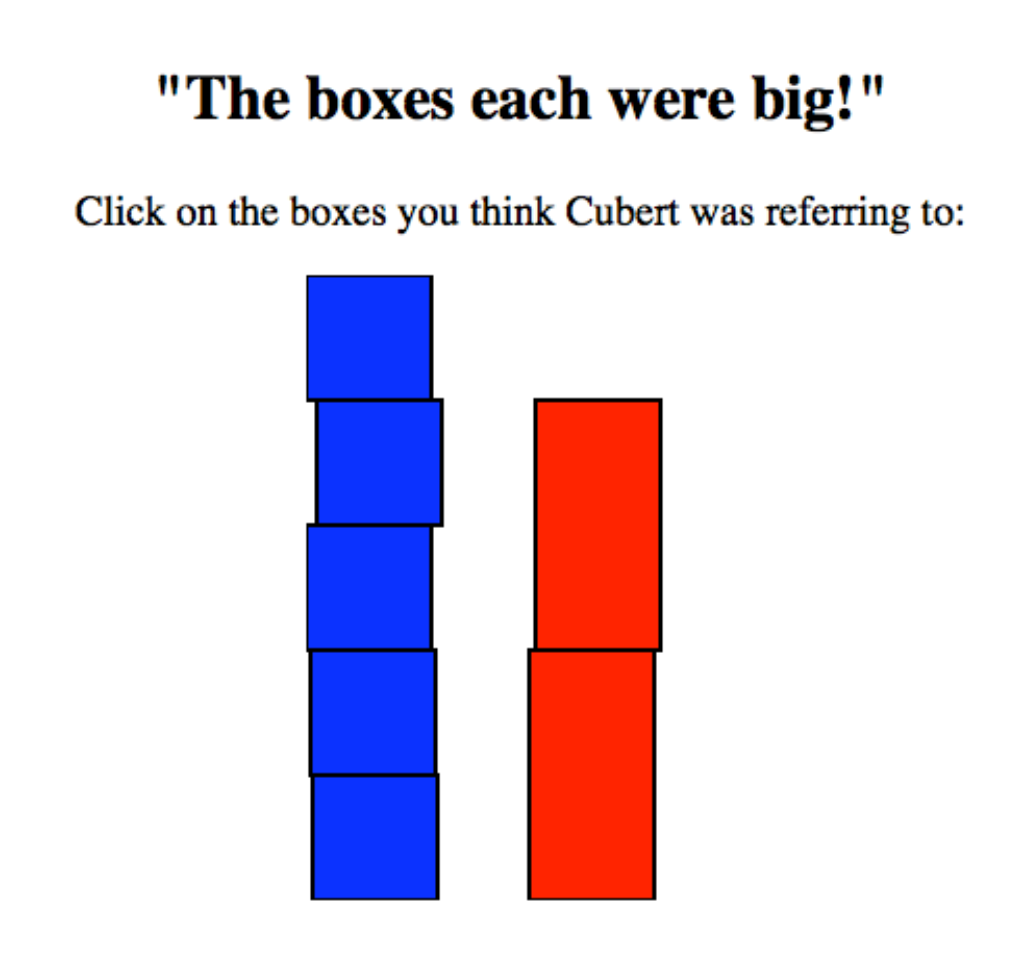
\includegraphics[width=3in]{images/trial2.eps}
	\caption{Example trial from Expt.~1 with the predicate \emph{big} in the ``each'' utterance.}\label{expt1trial}
\end{figure}

 Cubert used three predicates, \emph{big}, \emph{heavy}, and \emph{tall}, in three sentence frames, or utterances: bare \Last[a], ``each'' \Last[b], and ``together'' \Last[c]. Subjects saw each version of each predicate in a random order, completing nine trials. 

\subsubsection{Predictions}

If \emph{each} and \emph{together} are clear disambiguators for plural predication, we should should find a split in the choice of referent depending on which of these words appears. Encountering distributive \emph{each}, as in \ref{each}, subjects should choose the distributive referent (Fig.~\ref{expt1trial}, right); with collective \emph{together}, \ref{together}, subjects should choose the collective referent (Fig.~\ref{expt1trial}, left). 

For the potentially ambiguous bare utterances, stubbornly distributive \emph{big} ought to always prefer distributive referents. If predicating size and shape determines stubborn distributivity, \emph{tall} should pattern with \emph{big} in its stubborn distributivity. Given that size and height are visually assessable properties, the scenario manipulation should have no effect on Cubert's epistemic state, and therefore no effect on the resulting interpretations for bare \emph{big} and \emph{tall}. For complaisantly collective \emph{heavy}, we should find higher rates of collective referent choice for the bare utterance. And given that Cubert would need to lift individual boxes to assess their individual weight, to the extent that we find any effect of our scenario manipulation, we should we should find it for \emph{heavy}: moving all the boxes (as opposed to inspecting each box) would yield higher rates of collective referent choice, given the speakers limited access to individual box weights.

\subsubsection{Results}

Results were coded in terms of whether subjects chose the collective referent, and therefore the collective interpretation for Cubert's statement to Dot. Fig.\ \ref{results2} displays the proportion of collective choices, with bootstrapped 95\% confidence intervals \citep{diciccioefron1996}; a value of 1 indicates that participants chose the collective referent 100\% of the time.

To evaluate the disambiguating potential of our paraphrases, we first look at responses to these paraphrases, to the exclusion of the bare utterance. We fit a mixed effects logistic regression model \citep{baayenetal2008} using the \emph{lme4} package \citep{batesetal2014} in \emph{R}, predicting referent choice by \textsc{utterance} (``each,'' ``together''), as well as \textsc{trial} order.  The model included random intercepts for participants, predicates, and scenarios, as well as random slopes for participants grouped by \textsc{utterance} (i.e., the maximal random effects structure supported by the data). The full regression model appears in Appendix \ref{expt1results}. The model finds a main effect of \textsc{utterance} ($\beta$ = 5.50, $SE$ = 0.94, $z$ = 5.87, p $<$ 0.001); the effect of \textsc{trial} was not significant ($\beta$ = 0.06, $SE$ = 0.08, $z$ = 0.81, p $=$ 0.42). Thus, the ``together'' utterances yielded collective referent choices, and the ``each'' utterances did not.

To evaluate the behavior of the predicates in the absence of the disambiguating particles, together with the effect of our scenario manipulation, we next consider responses to the bare, potentially ambiguous utterance. We fit a mixed effects logistic regression model predicting referent choice by \textsc{predicate} (\emph{big}, \emph{heavy}, \emph{tall}), \textsc{scenario} (``move,'' ``inspect''), and \textsc{trial} order. The model included random intercepts and slopes for participants (grouped by \textsc{trial}; the maximal random effects structure supported by the data). The full regression model appears in Appendix \ref{expt1results}. The model finds mains effects of \textsc{predicate} for both \emph{heavy} ($\beta$ = 3.05, $SE$ = 1.23, $z$ = 2.48, p $<$ 0.05) and \emph{tall} ($\beta$ = 3.63, $SE$ = 1.29, $z$ = 2.82, p $<$ 0.01). Compared to \emph{big}, the other predicates yielded greater rates of collective referent choice. While the effect of \textsc{scenario} did not reach significance, we note the trend in Fig.~\ref{expt1results} whereby ``move'' scenarios tend to have higher rates of collective referent choice for bare \emph{heavy} utterances (34\% ``move'' vs.~14\% ``inspect''). A post-hoc t-test of this difference approaches significance ($t$ = -1.70, \emph{df} = 47.96, $p$ = 0.096).


\begin{figure}[h]
	\centering
	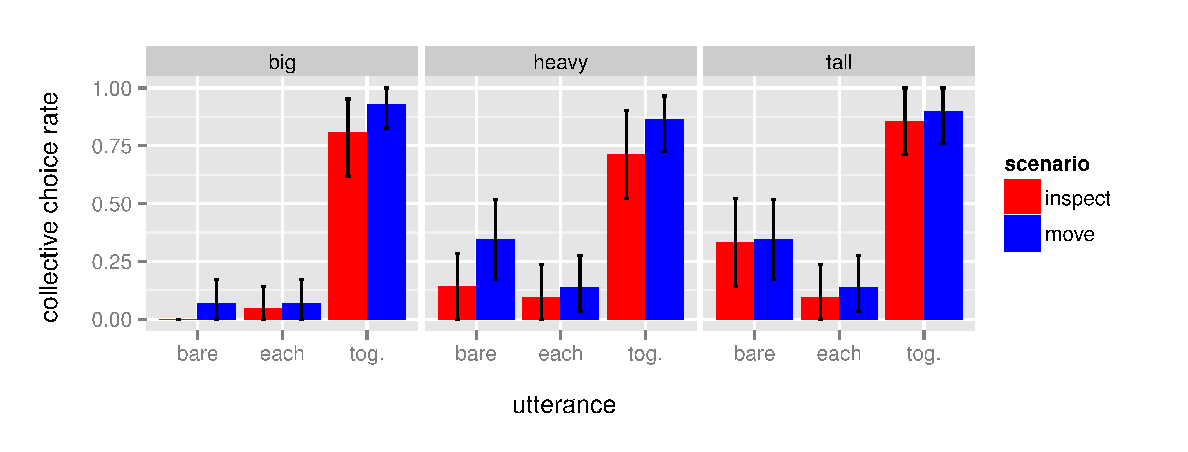
\includegraphics[width=\linewidth]{plots/expt1bootsci.eps}
	\vspace{-15pt}
	\caption{Proportion of collective choices.}\label{results2}
\end{figure}


\subsubsection{Discussion}

The disambiguating paraphrases behave as expected: \emph{each} delivers a distributive interpretation and \emph{together} delivers collective. We also find that the bare form of \emph{big} patterns differently from \emph{heavy} and \emph{tall} --- it is more distributive. This finding is expected with respect to \textit{big} vs.~\textit{heavy} (the former should be stubbornly distributive), but surprising given the behavior of \textit{tall}: both \emph{tall} and \emph{big} are predicates of size and shape. If naming properties of physical extent mediates the choice between distributive and collective interpretations of plural predications, we should find that \emph{tall} patterns with \emph{big}. Equally damning is the comparison between \emph{tall} and \emph{heavy}: if anything, \emph{tall} more consistently delivers collective interpretations. What allows \emph{tall} to readily receive collective interpretations --- while precluding them for \emph{big} --- in our experimental context? 

As discussed above, one candidate factor is the contextual predictability of the collective property: how easy it is for speakers and listeners to arrive at the same collective property for a given set of objects. We have seen that collective weight is a stable property of sets, which stands to explain the complaisance of \emph{heavy} toward collective interpretations. In the context of the current experiment, collective height is also predictable: boxes always appeared stacked one on top of the other, yielding stable total set heights. Collective size, however, could vary depending on the strategy used to evaluate it (height? width? area? volume?), thus accounting for the lack of collective interpretations for bare \emph{big}. In Expt.~2, we use the paraphrase methodology to directly investigate the role of contextual predictability in plural predication.

The results of the current experiment also highlight the role of speaker knowledge in plural predication: based solely on whether the context scenario had Cubert move vs.~inspect the boxes he received, we see a trend whereby bare \emph{heavy} received more or less collective interpretations, respectively. The absence of the effect for \emph{big} and \emph{tall} suggests an explanation in terms of the epistemic state of the speaker: in \textsc{move} scenarios the speakers is less likely to have access to individual box weights; the listener is therefore less likely to assume that the speaker, Cubert, intended a distributive interpretation for which he lacks evidence. We follow up on this result with a similar scenario manipulation in Expt.~2.

\subsection{Experiment 2: Manipulating context}

If physical arrangements are less likely to change, collective properties become more predictable, so collective interpretations stand a better chance of being informative. These interpretations should therefore become more likely. If speakers lack knowledge for one of two possible interpretations, the epistemically-supported interpretation should become more likely. In Expt.~2, we manipulated predictability and speakers' access to knowledge through a series of context scenarios, and used paraphrase endorsements to test the availability of collective interpretations.

\subsubsection{Participants}

We recruited 80 participants through Amazon's Mechanical Turk. Participants were compensated for participation.

\subsubsection{Design and methods}

The experimental context was similar to that of Expt.~1. Participants were first introduced to an agent, Cubert, who works in a factory with boxes. Cubert receives boxes from a dispenser in the ceiling. Participants began by observing the dispenser in action.

Between subjects, we manipulated the \textsc{scenario} story (``move'' vs.~``inspect''): Cubert's job was either to move shipments of boxes, or to inspect them. As in Expt.~1, in \textsc{move} scenarios, Cubert appeared with a dolly with which to carry the boxes. In \textsc{inspect} scenarios, Cubert appeared without a dolly.

Also between subjects, we manipulated the variability of \textsc{context} (``regular'' vs.~``random''). In regular contexts, the dispenser consistently stacked boxes on top of each other (Fig.~\ref{expt2context}, left). In random contexts, boxes were dispensed without any consistent physical arrangement (Fig.\ \ref{expt2context}, right). Participants saw four each of either regular or random context priming scenarios.

\begin{figure}[h]
\centering
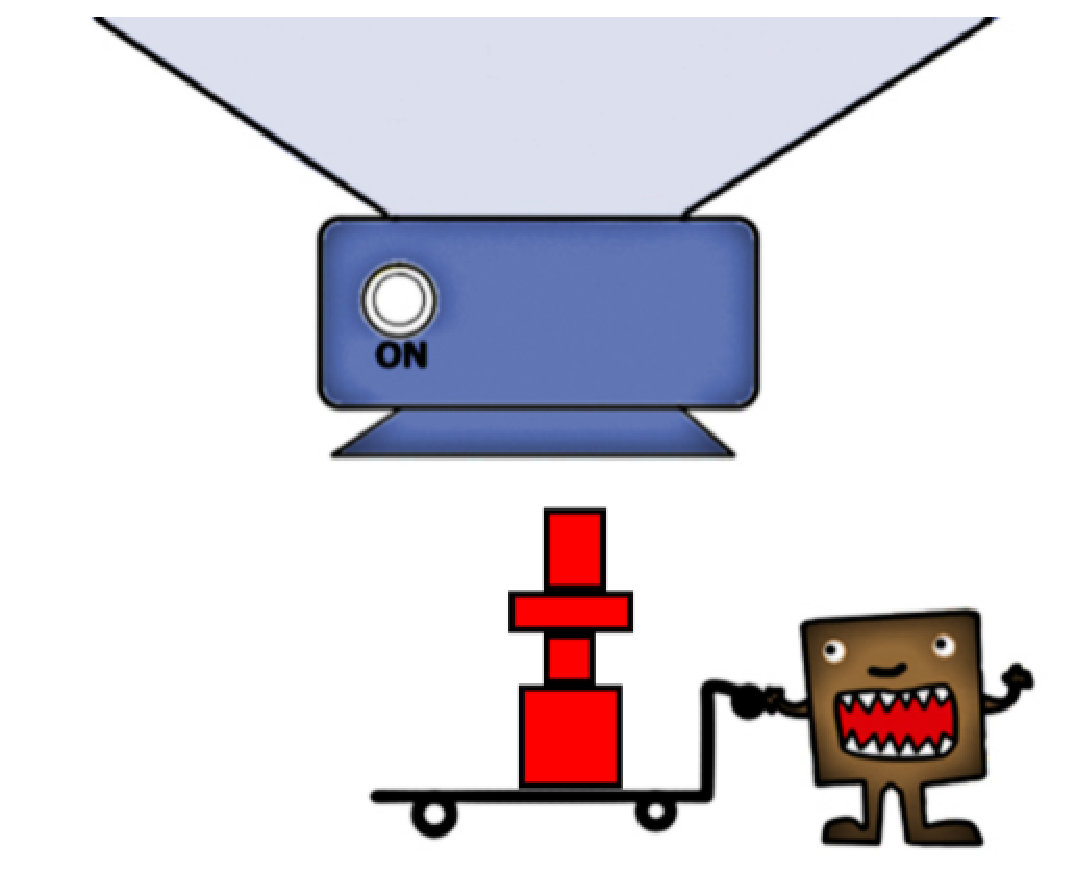
\includegraphics[width=.45\textwidth]{images/context13reg.eps}
\ \ \ \ 
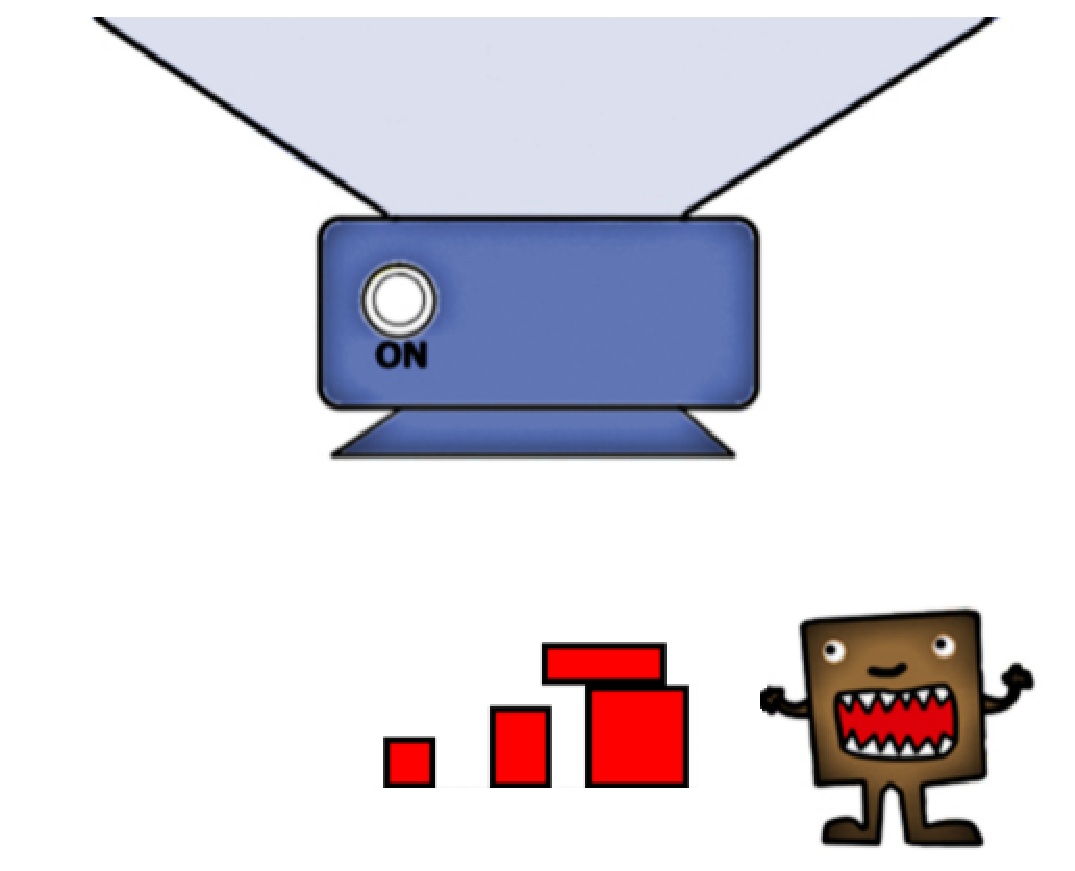
\includegraphics[width=.45\textwidth]{images/context13nodolly.eps}
\caption{Example context scenarios from Expt.~2. Left: the outcome of a ``regular,'' ``move'' context scenario. Right: the outcome of a ``random,'' ``inspect'' context scenario.\label{expt2context}}
\end{figure}


After observing the dispenser in action via the context  scenarios, participants were then introduced to a second agent, Dot, whom Cubert told about the boxes he moved/inspected. Participants were tasked with helping Dot understand what Cubert meant by his utterance. To do so, they saw an utterance and rated potential paraphrases on a sliding scale. The paraphrases were either distributive (with  ``each'') or collective (with ``together'').  Scale endpoints corresponded to whether the paraphrase was ``definitely'' or ``definitely not'' what Cubert meant by his utterance (Fig. \ref{trial}). Participants completed three trials in a random order with three different predicates: \emph{big}, \emph{heavy}, and \emph{tall}.


\begin{figure}[h]
\centering
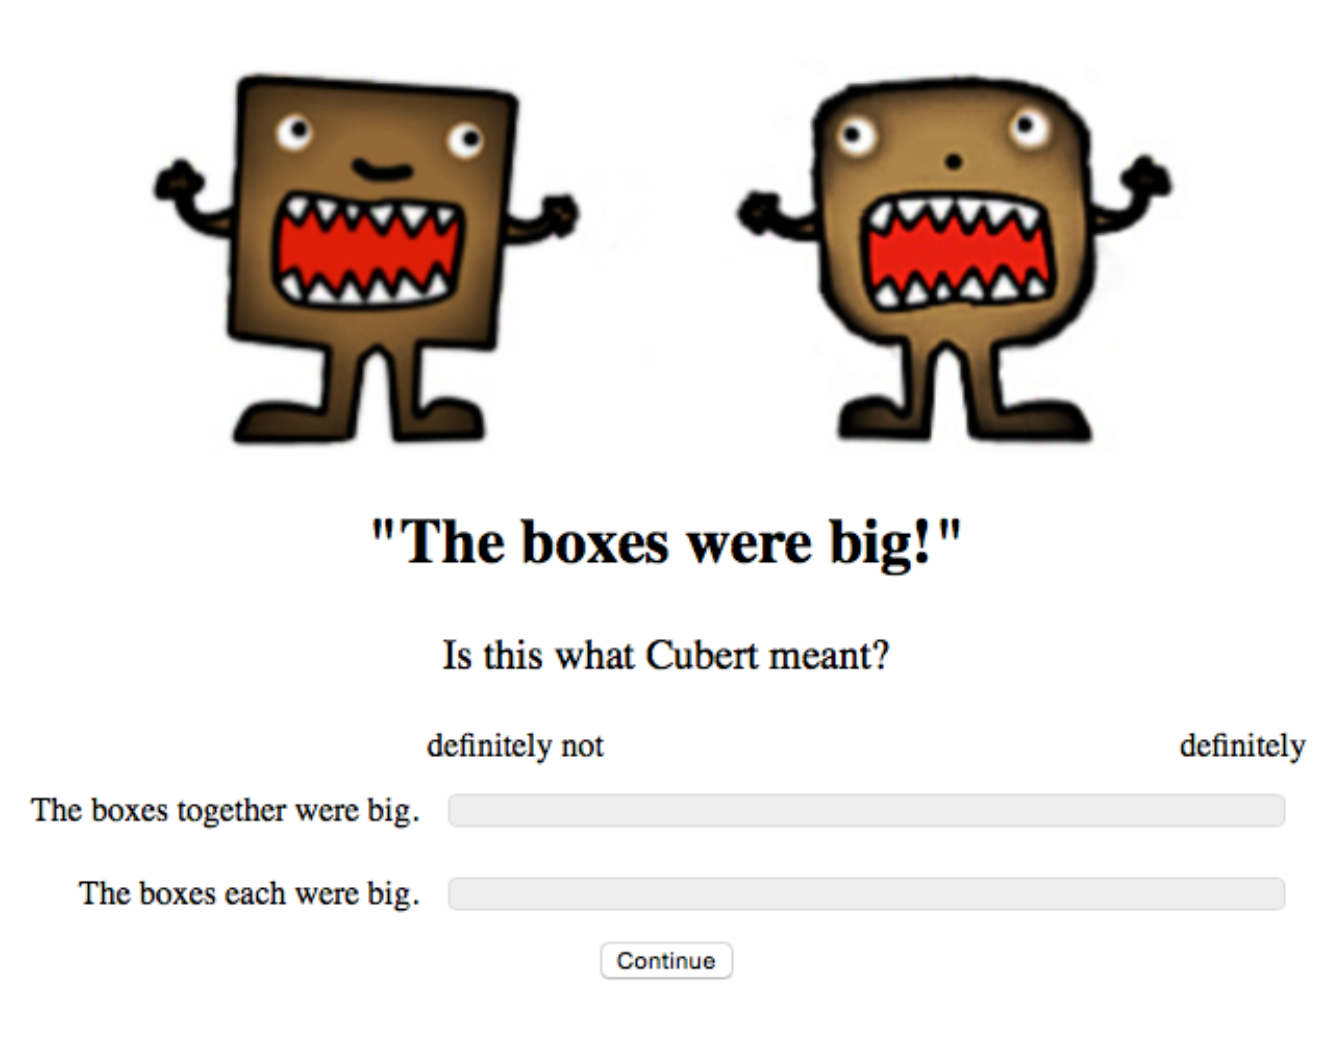
\includegraphics[width=4.5in]{images/trial.eps}
\caption{Example ``big'' trial.}\label{trial}
\end{figure}

\subsubsection{Predictions}

If contextual predictability of collective properties influences the availability of collective interpretations, we should find that regular arrangement contexts yield more collective interpretations, resulting in higher endorsement rates for the collective paraphrase with \emph{together}. This effect ought to hold for the predicates \emph{big} and \emph{tall} --- \emph{heavy} is already strongly contextually predictable, so we might not be able to increase its predictability --- but \emph{tall} should be the most sensitive to our context manipulation because it introduces regularity into its dimension of measurement directly: stacking boxes on top of each other to make collective height particularly salient.

Given the trending effect of speaker access to knowledge with \emph{heavy} in Expt.~1 --- where \emph{move} scenarios had greater rates of collective interpretations --- we should find a similar effect here: collective paraphrase endorsement for \emph{heavy} should be greater than distributive endorsement in \emph{move} scenarios, independent of the regularity of the context. We have no reason to expect a similar effect for the other two predicates, due to the visual assessability of their corresponding properties and their insensitivity to the scenario manipulation in Expt.~1.

\subsubsection{Results}

Fig.\ \ref{resultsexpt2} displays the raw paraphrase endorsement ratings averaged across all trials with bootstrapped 95\% confidence intervals. For the purpose of analysis, we analyze responses to the collective paraphrases (i.e., the red bars in Fig.~\ref{expt2results}); high rates of endorsement for the collective paraphrase signal greater rates of collective interpretation.\footnote{All reported results hold if instead we look at normalized collective paraphrase endorsement ratings (i.e., the difference between collective and distributive endorsements for each trial).} %calculated the difference between collective and distributive paraphrase endorsement ratings for each trial; Fig.~\ref{normresultsexpt2} presents these difference scores, where greater values of the difference score signal greater rates of collective paraphrase endorsement.

\begin{figure}[h!]
	\centering
	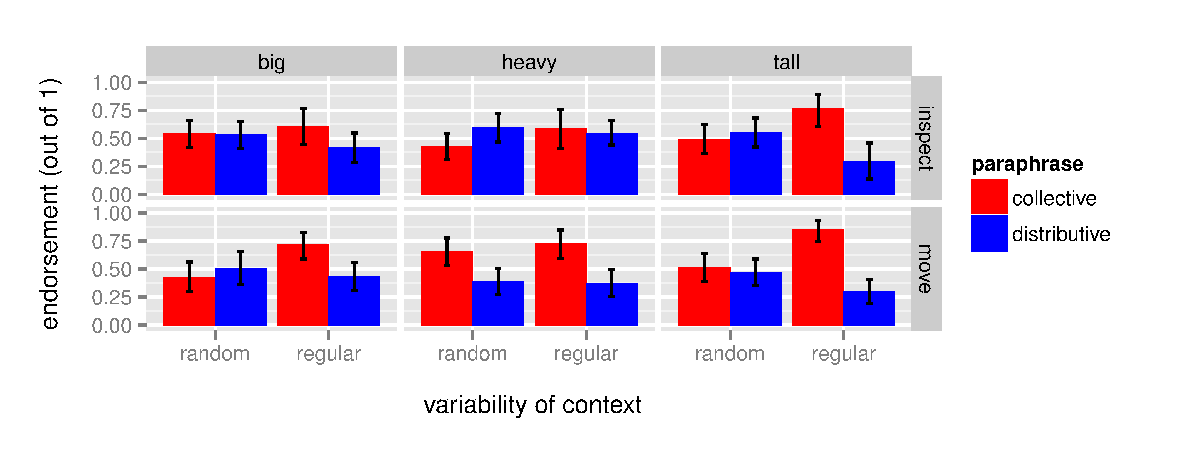
\includegraphics[width=\linewidth]{plots/expt2rawbootsci.eps} 
	\vspace{-15pt}
	\caption{Paraphrase endorsement rate averaged across all trials in Expt.~2.}\label{resultsexpt2}
\end{figure}


We fit a linear mixed effects model predicting collective endorsement ratings by \textsc{context} (random vs.~regular),
\textsc{predicate} (\emph{big}, \emph{heavy}, \emph{tall}),
 \textsc{scenario} (``inspect'' vs.~``move''), and \textsc{trial} order; the model included interactions between \textsc{predicate} and \textsc{context}, and between \textsc{predicate} and \textsc{scenario}. The model also included random intercepts for participants, as well as random slopes for participants grouped by \textsc{trial}. The full regression model appears in Appendix \ref{expt2results}.

As demonstrated in Fig.~\ref{resultsexpt2}, there was a main effect of \textsc{context}, so that for all predicates regular contexts had more collective interpretations than did random contexts ($\beta$ = 0.18, $SE$ = 0.07, $t$ = 2.70, p $<$ 0.01). The model finds a main effect of the predicate \emph{tall} ($\beta$ = 0.07, $SE$ = 0.04, $t$ = 2.00, p $<$ 0.05), driven in large part by a marginally significant interaction between \emph{tall} and \textsc{context} ($\beta$ = 0.13, $SE$ = 0.08, $t$ = 1.72, p $=$ 0.09): \emph{tall} was most affected by our contextual manipulation, yielding the greatest rates of collective interpretations in regular contexts. Finally, the model finds a significant interaction between the predicate \emph{heavy} and \textsc{scenario} ($\beta$ = 0.21, $SE$ = 0.08, $t$ = 2.77, p $<$ 0.01): \emph{heavy} received more collective interpretations in ``move'' scenarios.

\subsubsection{Discussion}

As we would expect if contextual predictability of collective properties determines the viability of collective interpretations, regular contexts had higher ratings for collective paraphrases and lower ratings for distributive ones. The predicate \textit{tall} was most affected by our contextual manipulation, which directly targeted the height dimension, stacking boxes on top of each other. But \emph{big}, claimed to be stubbornly distributive, is similarly affected: regular contexts yield more collective interpretations. 

While the predicate \emph{heavy} was affected by contextual variability, most notable is its sensitivity to the ``move'' vs.~``inspect'' scenario manipulation: as was the trend in the results of Expt.~1, ``move'' scenarios yielded much greater collective endorsement ratings for \emph{heavy}. This manipulation privileges collective interpretations by limiting speakers' access to the information they would need to verify a distributive interpretation; Cubert lacked access to individual box weights in ``move'' scenarios. The predicates \emph{big} and \emph{tall} were not affected by the speaker knowledge scenario manipulation because they name properties that are visually assessable, and thus visually accessible.

Taken together, our results demonstrate the central role of context in plural predication: as collective properties become more predictable, collective interpretations become more likely; and without epistemic support, distributive interpretations become less likely. These findings support a pragmatic account of stubborn distributivity according to which ostensibly stubbornly distributive predicates are such because the properties they name are unpredictable, or unstable in context. Next, we formalize this choice of interpretation in a Bayesian Rational Speech-Act model \citep{frankgoodman2012,lassitergoodman2013}. Noisy (i.e., more variable) interpretations are less useful because they require more coordination between speakers and listeners; they are therefore less likely. Similarly, listeners are less likely to assume interpretations for which speakers lack knowledge.



\section{Modeling plural predication}

We have seen that disambiguating plural predication depends not only on local linguistic context (e.g., the predicate, its subject, and disambiguating particles like \emph{each} or \emph{together}), but also on the broader discourse context. Moreover, we showed how properties of the broader context stand to explain the effect certain predicates have on disambiguating plural predication: Complaisantly collective predicates like \emph{heavy} name collective properties that are stable and predictable on the basis of context; stubbornly distributive predicates like \emph{big} name collective properties that are unstable and unpredictable on the basis of context. The less predictable the collective property, the noisier the collective interpretation. Conversely, we saw that increasing contextual predictability increases collective interpretations, presumably by decreasing potential interpretation noise. A noisy interpretation is less useful at communicating its intended message, and therefore less likely. Additionally, we saw that listeners track speaker knowledge as they disambiguate plural predication, so that unsupported interpretations are unlikely. To formalize the effect of contextual predictability and speaker access to knowledge in plural predication, we adopt a lifted variable variant of the Bayesian Rational Speech-Act model. 

The Rational Speech-Act (RSA) framework views communication as recursive reasoning between a speaker and a listener. The listener interprets the speaker's utterance by reasoning about a cooperative speaker trying to inform a naive listener about some state of affairs. Using Bayesian inference, the listener infers what the state of the world is likely to be given that a speaker produced some utterance, knowing that the speaker is reasoning about how a listener is most likely to interpret that utterance. Thus, we have at least three levels of inference. At the top, the sophisticated, pragmatic listener, \emph{L}$_{1}$, reasons about the pragmatic speaker, \emph{S}$_{1}$, and infers the state of the world \emph{s} given that the speaker chose to produce the utterance \emph{u}. The speaker chooses \emph{u} by maximizing the likelihood that a naive, literal listener, \emph{L}$_{0}$, would correctly infer the state of the world \emph{s} given the literal meaning of \emph{u}.

In more detail, the pragmatic listener \emph{L}$_{1}$ computes the probability of a state \emph{s} given some utterance \emph{u}. By reasoning about the speaker \emph{S}$_{1}$, this probability is proportional to the probability that \emph{S}$_{1}$ would choose to utter \emph{u} to communicate about the state \emph{s}, together with the prior probability of \emph{s} itself.

\ex. \emph{The pragmatic listener}:\\
$P_{L_{1}}(s|u) \propto P_{S_{1}}(u|s) \cdot P(s)$

The speaker \emph{S}$_{1}$ desires to choose an utterance \emph{u} that would most effectively communicate some state \emph{s} to a hypothesized literal listener \emph{L}$_{0}$.  In other words, \emph{S}$_{1}$ wants to minimize the effort \emph{L}$_{0}$ would need to arrive at \emph{s} from \emph{u}, all while being efficient at communicating. This trade-off between efficacy and efficiency is not trivial: speakers could always use minimal ambiguity, but unambiguous utterances tend toward the unwieldy, and, very often, unnecessary. \emph{S}$_{1}$ thus seeks to minimize the surprisal of \emph{s} given \emph{u} for the literal listener \emph{L}$_{0}$, while bearing in mind the utterance cost, \emph{C}(\emph{u}). In \Next, we formalize the speaker's utility function \emph{U}$_{S_{1}}$: utterances are more useful at communicating about some state as surprisal and utterance cost decrease.

\ex. \emph{The speaker's utility function}:\\
$U_{S_{1}}(u;s) = \textrm{log}L_{0}(s|u) - C(u)$

With this utility function in mind, $S_{1}$ computes the probability of an utterance $u$ given some state $s$ in proportion to the speaker's utility function. The term \mbox{$\alpha > 0$} controls the speaker's optimality, that is, the speaker's rationality in choosing utterances. ($\alpha$ corresponds to the temperature parameter of $S_{1}$'s soft-max optimization.)

\ex. \emph{The pragmatic speaker}:\\
$P_{S_{1}}(u|s) \propto \textrm{exp}(\alpha U_{S_{1}}\!(u;s))$

At the base of this reasoning, the naive, literal listener $L_{0}$ interprets an utterance according to its meaning. That is, $L_{0}$ computes the probability of $s$ given $u$ according to the semantics of $u$ and the prior probability of $s$. A standard view of the semantic content of an utterance suffices: a mapping from states of the world to truth values.

\ex. \emph{The literal listener}:\\
$P_{L_{0}}(s|u) \propto \sem{u}(s) \cdot P(s)$

Within the RSA framework, communication is thus modeled as in Fig.~\ref{RSA}, where $L_{1}$ reasons about $S_{1}$'s reasoning about a hypothetical $L_{0}$.

\begin{figure}[h]
	%\psset{rowsep=20pt,colsep=50pt,nodesep=4pt} 
	\centering	
		\psset{arrows=->,rowsep=10pt,colsep=10pt,nodesep=2pt} \begin{psmatrix}
			\rnode[b]{l1}{$L_{1}$} & \emph{pragmatic listener} & $P_{L_{1}}(s|u) \propto P_{S_{1}}(u|s) \cdot P(s)$\\
			\rnode[c]{s1}{$S_{1}$} & \emph{pragmatic speaker}
			& $P_{S_{1}}(u|s) \propto \textrm{exp}(\alpha U_{S_{1}}\!(u;s))$ \\
			\rnode[t]{l0}{$L_{0}$} & \emph{literal listener} & $P_{L_{0}}(s|u) \propto \sem{u}(s) \cdot P(s)$
			\ncline{l1}{s1} 
			\ncline{s1}{l0} 
		\end{psmatrix}
	\caption{Graphical representation of the Bayesian RSA model.}\label{RSA}
\end{figure}

In its initial formulation, \citet{frankgoodman2012} use the basic RSA framework to model referent choice in efficient communication. To see the mechanism at work, imagine a referential communication game with three objects, as in Fig.~\ref{refgame}. Suppose a speaker wants to signal an object, but only has a single word with which to do so.
Applying the RSA model schematized in Fig.~\ref{RSA} to the communication scenario in Fig.~\ref{refgame}, the speaker $S_{1}$ chooses a word $u$ to best signal an object $s$ to a literal listener $L_{0}$, who interprets $u$ in proportion to the prior probability of naming objects in the scenario (i.e., to an object's salience, $P(s)$). The pragmatic listener $L_{1}$ reasons about the speaker's reasoning, and interprets $u$ accordingly.  By formalizing the contributions of salience and  efficiency, the RSA framework provides an information-theoretic definition of informativeness in pragmatic inference. This definition will prove crucial in understanding the contribution of contextual predictability of collective properties in the interpretation of plural predication.

Continuing with the language game in Fig.~\ref{refgame}, suppose you are the speaker and you want to signal the object in the center to a listener. Your options for $u$ are the words ``blue'' and ``circle''. XXX demonstration of the basic RSA success

\begin{figure}[h]
\centering
		\includegraphics[width=.4\linewidth]{images/communication-game.eps}
		\caption{Example referential communication scenario from \citet{frankgoodman2012}. Speakers choose a single word, $u$, to signal an object, $s$.}\label{refgame}
\end{figure}

To successfully model ambiguity resolution in plural predication, we need to adopt a variant of the RSA approach wherein speakers and listeners reason not merely over utterances and meanings, but also over variables that contribute to those meanings. This sort of ``lifted variable'' (also called ``lexical uncertainty'') RSA model has proven useful in accounts of adjective semantics (where the lifted variable is the adjective's degree threshold; \citealp{lassitergoodman2013}), specificity implicatures (where the lifted variable determines the choice of lexica; \citealp{bergenetal2012}), and non-literal meaning (where the lifted variable concerns the dimension along which the speaker intends to communicate; \citealp{kaoetal2014}), to name just a few applications (see also XXX). Here, the lifted variable about which speakers and listeners reason determines the interpretation of an ambiguous plural predication: whether an utterance is interpreted collectively or distributively.

The ambiguity-resolving free variable $V$ determines the interpretation of an plural predication utterance $u$. When $V$ is \textsc{collective}, $u$ receives a collective interpretation; when $V$ is \textsc{distributive}, $u$ receives a distributive interpretation. Now, the lifted variable literal listener $L_{0}$ computes the probability of some state $s$ given an utterance $u$ and some value for $V$. 

\ex. \emph{The lifted variable literal listener}:\\
$P_{L_{0}}(s|u,V) \propto \sem{u}^{V}(s) \cdot P(s) \cdot P(V)$

But $L_{0}$ does not know the value of $V$. Put differently, the literal listener does not know the intended interpretation of an ambiguous utterance. The name "lifted variable RSA" captures the fact that this free variable gets passed up from the literal listener through the speaker to be estimated by the pragmatic listener; the pragmatic listener fixes the interpretation by which the literal listener interprets the utterance.

The lifted variable pragmatic speaker $S_{1}$ now incorporates $V$ so that utterances are chosen to best communicate some state $s$ given an interpretation $V$. $S_{1}$ maximizes the likelihood of $u$ given $s$ and $V$, relative to the speaker utility function which minimizes surprisal and the cost of $u$.

\ex. \emph{The lifted variable speaker's utility function}:\\
$U_{S_{1}}(u;s,V) = \textrm{log}L_{0}(s|u,V) - C(u)$

\ex. \emph{The lifted variable pragmatic speaker}:\\
$P_{S_{1}}(u|s,V) \propto \textrm{exp}(\alpha U_{S_{1}}\!(u;s,V))$

At the top level, the lifted variable pragmatic listener $L_{1}$ interprets an utterance $u$, inferring the state $s$ and resolving the variable $V$. $L_{1}$ now reasons about the speaker, who presumably has an interpretation (i.e., a value for V) in mind.

\ex. \emph{The lifted variable pragmatic listener}:\\
$P_{L_{1}}(s,V|u) \propto P_{S_{1}}(u|s,V) \cdot P(s) \cdot P(V)$

To capture the speaker's epistemic state, our model needs one last element. Following \cite{goodmanstuhlmuller2013}, we include a parameter $a$ determining the speaker's possibly incomplete access to the world state $s$. Now, the speaker makes an observation $o$ about the state $s$, and, depending on the speaker's perceptual access $a$, $o$ might be identical to $s$ (i.e., the speaker has full access to information about the state) or a summary of $s$ (say, its sum, corresponding to the speaker's only having access to total size or weight of the state). From the observation $o$ and his perceptual access $a$, the speaker generates an expectation about the states $s$ that $o$ might have been an observation of. For example, if the speaker only has perceptual access the sum of some state (e.g., total weight), the speaker would infer a distribution over the possible individual properties that could have generated that observation (e.g., the weights of individual boxes). The speaker thus selects an utterance $u$ to convey information about the likely state $s$ that generated the observation $o$. The revised  pragmatic speaker model, \Next, takes into account perceptual access and potential uncertainty about the world state. Here, the pragmatic speaker calculates a believe distribution over what the actual state $s$ would be given the observation $o$ and perceptual access $a$: $P(s|o,a)$.

\ex. $P_{S_{1}} (u|o,a,V) \propto \textrm{exp}(\alpha \mathbb{E}_{P(s|o,a)}[U_{S_{1}} (u;s,V)])$

Where speaker's access to knowledge is shared between speakers in listeners (in our experimental setting, participants knew whether Cubert moved the boxes together or inspected each individually), $a$ is shared between $S_{1}$ and $L_{1}$. The full lifted variable RSA model of plural predication appears in Fig.~\ref{pluralRSA}.

\begin{figure}[h]
	%\psset{rowsep=20pt,colsep=50pt,nodesep=4pt} 
\centering
		\psset{arrows=->,rowsep=10pt,colsep=10pt,nodesep=2pt} \begin{psmatrix}
			\rnode[b]{l1}{$L_{1}$} & \emph{pragmatic listener} & $P_{L_{1}}(s,V|u,a) \propto P_{S_{1}}(u|s,a) \cdot P(s) \cdot P(V)$\\
			\rnode[c]{s1}{$S_{1}$} & \emph{pragmatic speaker} &
			$P_{S_{1}} (u|o,a,V) \propto \textrm{exp}(\alpha \mathbb{E}_{P(s|o,a)}[U_{S_{1}} (u;s,V)])$ \\
			\rnode[t]{l0}{$L_{0}$} & \emph{literal listener} & $P_{L_{0}}(s|u,V) \propto \sem{u}^{V}(s) \cdot P(s) \cdot P(V)$
			\ncline{l1}{s1} 
			\ncline{s1}{l0} 
		\end{psmatrix}
	\caption{The full Bayesian RSA plural predication model. $L_{1}$ infers the state $s$ and an interpretation-resolving variable $V$ given an utterance $u$ and the speaker's perceptual access $a$ to $s$. $S_{1}$ chooses $u$ given an observation $o$ of $s$, certain access $a$ from $o$ to $s$, and an intended interpretation $V$ of $u$. $L_{0}$ infers the state $s$ given some utterance $u$ and its interpretation $V$.} \label{pluralRSA}
\end{figure}

 To summarize: the pragmatic listener resolves ambiguity while interpreting an utterance by reasoning about the pragmatic speaker, who chooses utterances most likely to communicate some state via a specific interpretation to a naive, literal listener. The speaker and pragmatic listener track the speaker's access to knowledge, which determines whether the speaker has limited access to the state about which he communicates. In other words, listeners reason about likely interpretations of ambiguous plural predications given their intuitive understanding of speakers and their prior knowledge of the world (i.e., which states and interpretations are \emph{a priori} likely).

To generate qualitative and quantitative predictions that we may compare with our experimental results, we need to fix various parameter settings within the model. Here we fill in more details of these settings, with the caveat that the qualitative model results presented below are robust to a broad range of parameter settings; the specific values we give here are used merely to demonstrate the general behavior and success of the model.\footnote{XXX specifics about the range of parameter settings that are possible, and the settings that are not.}

 States $s$ correspond to sets of four objects, which hold scalar properties. More specifically, states are sets of positive integers, for example $\{3, 3, 4, 4\}$ or $\{3, 4, 4, 4\}$. Taking these objects as stand-ins for boxes and their properties as stand-ins for individual box sizes, the state $\{3, 3, 4, 4\}$ corresponds to a plurality of four boxes, two of size 3 and two of size 4. States are formed by drawing four times from a uniform prior distribution over boxes (i.e., objects); boxes come in two sizes: 3 or 4.
 
 Next, the utterances. Speakers have the choice between three utterances: one {unambiguously distributive} (e.g., \emph{the boxes each are big}), one {unambiguously collective} (e.g., \emph{the boxes together are big}), and the last {ambiguous} between a distributive and collective interpretation (e.g., \emph{the boxes are big}). The ambiguous utterance is always as least as cheap (in terms of the cost to the speaker) as the unambiguous utterances. In \Next, we give the semantics for these utterances, to be used in our model by the literal listener $L_{0}$.
 
 \ex. \emph{Utterance semantics}:
 \a. \sem{\texttt{distributive}} = \lam $s$. \texttt{distributive-interpretation}($s$)
 \b. \sem{\texttt{collective}} = \lam $s$. \texttt{collective-interpretation}($s$)
 \b. \sem{\texttt{ambiguous}} = \lam $V$\lam $s$. \texttt{if} $V$ = \textsc{collective}, \texttt{then}\\  \textcolor{white}{\sem{\texttt{ambiguous}} = \lam $V$\lam $s$. }\texttt{collective-interpretation}($s$)\\
 \textcolor{white}{\sem{\texttt{ambiguous}} = \lam $V$\lam $s$. }\texttt{else}, \\
 \textcolor{white}{\sem{\texttt{ambiguous}} = \lam $V$\lam $s$. }\texttt{distributive-interpretation}($s$)
 
 The \texttt{distributive} utterance receives a distributive interpretation. The \texttt{collective} utterance receives a collective interpretation. The interpretation of the \texttt{ambiguous} utterance depends on the value of the interpretation-resolving variable $V$, which the pragmatic listener infers. When $V$ is \textsc{collective}, the utterance receives a collective interpretation; otherwise, the utterance receives a distributive interpretation. These interpretations carry the semantics in \Next.
 
 \ex. \emph{Interpretation semantics}:
 \a. \sem{\texttt{distributive-interpretation}} =
\begin{flushright}\lam $s$. $\forall$x$\in$$s$[x $>$ \texttt{distributive-threshold}]\end{flushright}
\b. \sem{\texttt{collective-interpretation}} = 
\begin{flushright}\lam $s$. (\texttt{sum}($s$) $\times$ \textcolor{red}{\texttt{noise}}) $>$ \texttt{collective-threshold}\end{flushright}

The \texttt{distributive-interpretation} is true of a state $s$ just in case each of its members exceeds some distributive threshold.\footnote{Following \cite{lassitergoodman2013}, we treat the threshold parameters as lifted variables that get resolved by the pragmatic listener as he interprets the speaker's utterance. So, strictly speaker, $V$ in Fig.~\ref{pluralRSA} represents not just the interpretation-resolving variable, but also the threshold variables for the gradable predicates.} In our box setting, this semantics captures the fact that the distributive interpretation of a gradable predicate is true of a plurality when each of its members exceeds a contextually-determined cutoff \citep{kennedy1999,lassitergoodman2013}. The \texttt{collective-interpretation} is true of a state $s$ just in case the sum of that state --- the state taken together --- exceeds some collective threshold. Here we capture the sum-based aggregation inherent to collective interpretations of gradable predicates \citep{scha1984}. So far, no deviation from the formal semantics tradition.

What sets this semantics apart from the tradition that informs it is the \textcolor{red}{\texttt{noise}} parameter in the \texttt{collective-interpretation}, a scalar multiplier of the set aggregate estimate. This parameter explicitly represents possible noise in the determination of, say, collective size. For our purposes, lower noise (i.e., values closer to 1) corresponds to increased contextual predictability of the collective property. To evaluate the qualitative predictions of our model, we begin with the possible values for \textcolor{red}{\texttt{noise}} shown in \Next, where, for example, \texttt{low} \textcolor{red}{\texttt{noise}} equals 1 (i.e., no change to the state estimate) 100\% of the time.

\ex. \emph{Noise priors}:\\[5pt]
\texttt{no} \textcolor{red}{\texttt{noise}}:\\[2pt]
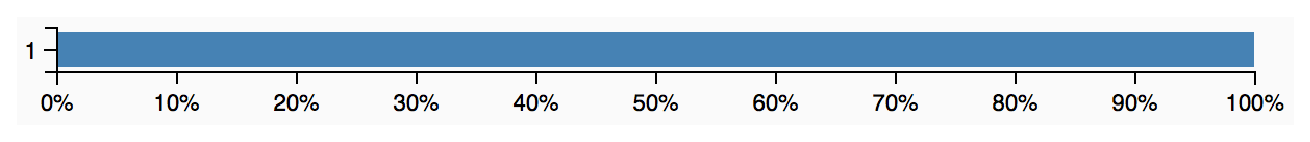
\includegraphics[width=\linewidth]{images/no-noise.eps}\\[5pt]
\texttt{low} \textcolor{red}{\texttt{noise}}:\\[2pt]
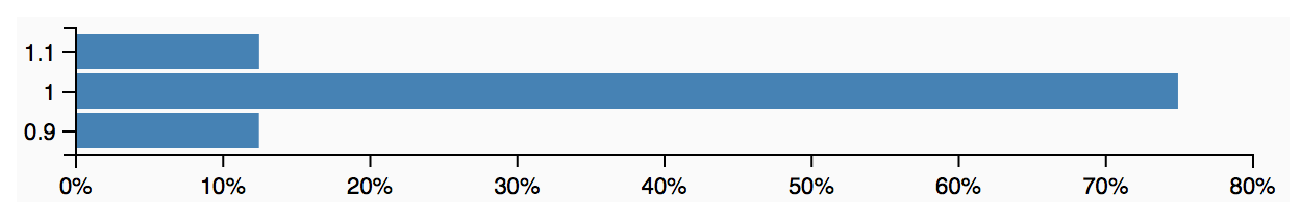
\includegraphics[width=\linewidth]{images/low-noise.eps}\\[5pt]
\texttt{medium} \textcolor{red}{\texttt{noise}}:\\[2pt]
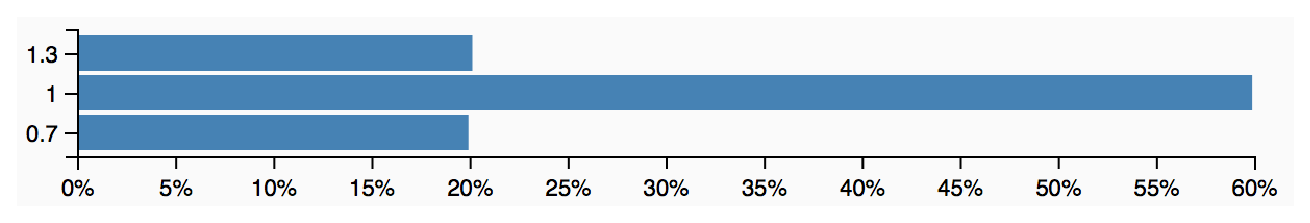
\includegraphics[width=\linewidth]{images/mid-noise.eps}\\[5pt]
\texttt{high} \textcolor{red}{\texttt{noise}}:\\[2pt]
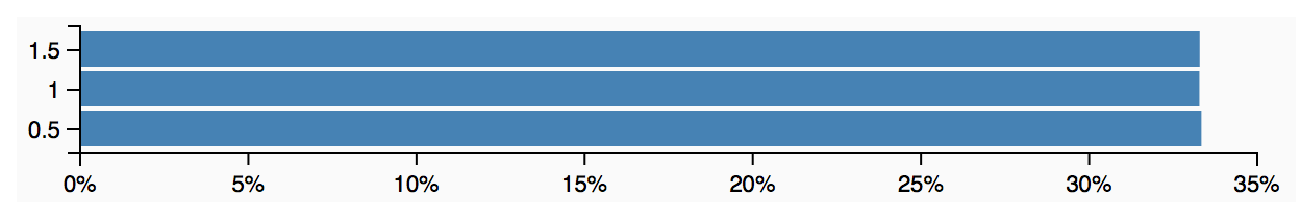
\includegraphics[width=\linewidth]{images/high-noise.eps}

With \texttt{no} noise, our estimates are spot on and collective properties are maximally predictable from context. Increasing noise, contextual predictability decreases: our estimates of collective properties deviate from the true state. Noise (i.e., contextual predictability) is a property of the discourse context, and as such speakers and listeners both have access to its value.

Lastly, to model speaker access to knowledge, the global parameter $a$ determines whether the speaker's state observation $o$ matches the state exactly (i.e., the speaker has full perceptual access to $s$), or whether it summarizes $s$ via summation (i.e., the speaker has limited perceptual access to $s$). Where $a$ is set to \texttt{full} knowledge, the speaker's belief distribution over possible states is exact, a delta distribution over \emph{the} state (Fig.~\ref{speakerbelief}, top). Having observed $\{3,3,4,4\}$, the speaker knows the state is $\{3,3,4,4\}$ (and not, say $\{4,4,3,3\}$). Where $a$ is set to \texttt{partial} knowledge, the speaker's belief distribution is broader (Fig.~\ref{speakerbelief}, bottom). With \texttt{partial} knowledge, the speaker only observes the sum of the individual state values, say 14. But more than one state could generate this value, namely any combination of two size 3 boxes with two size 4 boxes.

\begin{figure}[h]
	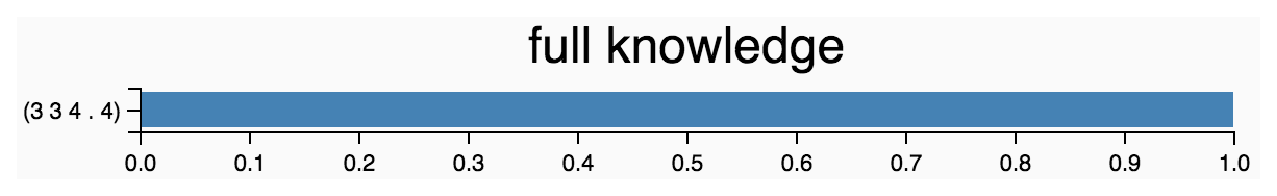
\includegraphics[width=\linewidth]{images/speaker-full.eps}\\
	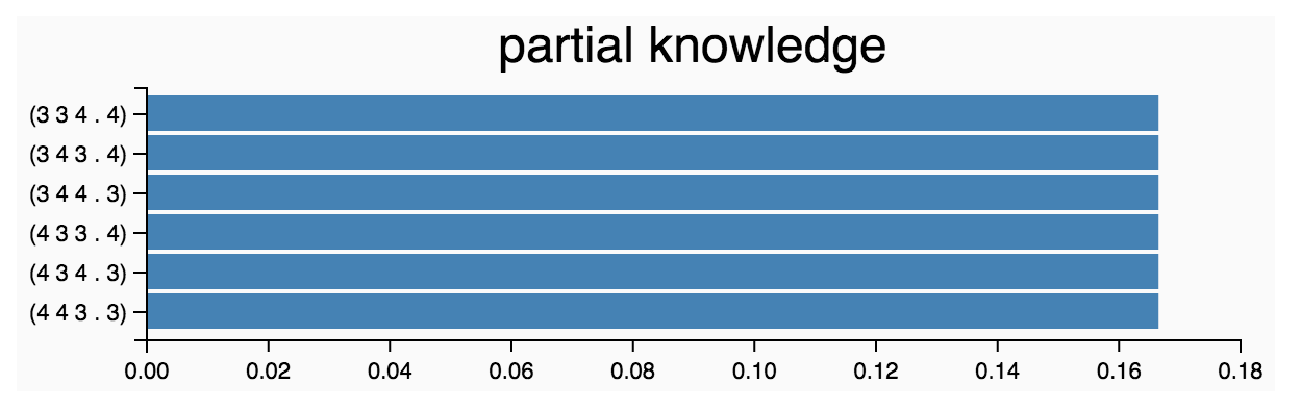
\includegraphics[width=\linewidth]{images/speaker-partial.eps}
	\caption{Speaker belief distributions resulting from \texttt{full} (top) and \texttt{partial} (bottom) perceptual access to the state $\{3,3,4,4\}$. XXX prettier plots} \label{speakerbelief}
\end{figure}

Finally, we have the pieces needed to generate predictions from the plural predication model. Given our interest in the effects of noise and speaker knowledge on the interpretation of potentially ambiguous plural predications, of primary interest is the value of the interpretation-resolving variable $V$ for the \texttt{ambiguous} utterance. In Fig.~\ref{modelresults}, we plot the probability that $V$ is \texttt{collective} after hearing the \texttt{ambiguous} utterance; in other words, we plot the probability of a collective interpretation as a function of collective noise and speaker knowledge.

\begin{figure}[h]
	\centering
	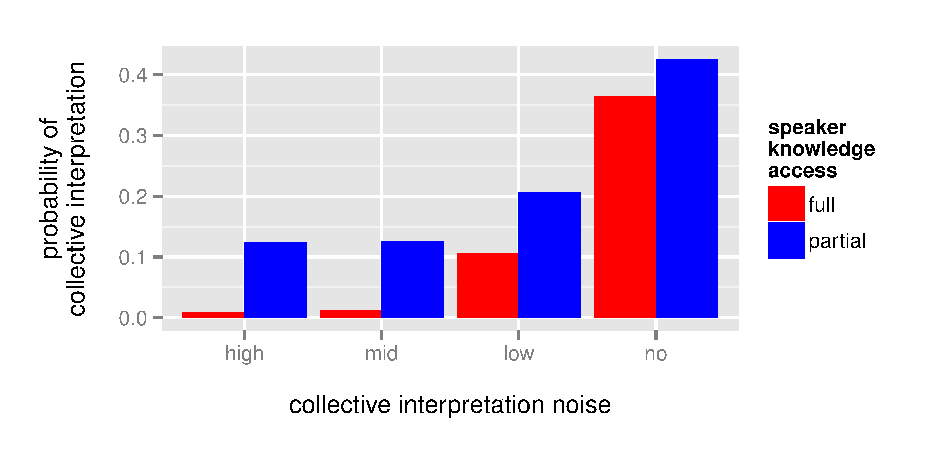
\includegraphics[width=\linewidth]{plots/model-results.eps}
	\vspace{-20pt}
	\caption{Model predictions for the probability of the \texttt{ambiguous} utterance receiving a collective interpretation as a function of collective interpretation noise and speaker knowledge access.} \label{modelresults}
\end{figure}

The qualitative predictions of our plural predication model match the intuitions and experimental results that motivated the model in the first place. Perhaps most striking is the monotonic increase in probability of collective interpretations as collective noise decreases. That is to say, as noise decreases, collective properties become more predictable in context, and collective interpretations become more likely. We now have a formal understanding as to why this effect holds: the noisier the collective interpretation, the less likely the listener $L_{0}$ is to correctly resolve the question under discussion, namely the properties of the named boxes $s$. Given that the speaker $S_{1}$'s goal is to successfully communicate $s$ to $L_{0}$, the noisier an interpretation, the less useful it is at achieving this goal; the speaker is therefore less likely to intend this interpretation, and as a result the pragmatic listener $L_{1}$ is less likely to infer it.

Another outcome of our model's predictions is the increase in the probability of a collective interpretation as the speaker's knowledge access becomes limited. With only partial access to the actual state $s$ --- such that the speaker's observation $o$ of $s$ is its summation ---  $S_{1}$ is less likely to have precise information concerning $s$ about which to communicate. $L_{1}$ tracks  $S_{1}$'s epistemic state, and therefore knows whether the speaker has full or partial knowledge. In the case of partial knowledge, a distributive interpretation lacks perceptual/epistemic support, and therefore becomes less likely; as a result, collective interpretations become more likely.

We have verified the qualitative predictions of our account of plural predication: increasing the contextual predictability of collective properties (by decreasing estimate noise) increases the probability of collective interpretation; and, regardless of the amount of collective noise, removing support for a distributive interpretation (by limiting speaker's access to individual properties) decreases the probability of a distributive interpretation and thus increases the probability of a collective interpretation. Crucially, both of these qualitative predictions are borne out while making minimal assumptions concerning model parameters. Once we fit these parameters to the human data collected in Expt.~2, we may test both qualitative and quantitative predictions of the model.

Comparing the model predictions in Fig.~\ref{modelresults} to the rates of collective endorsement from Expt.~2 in Fig.~\ref{expt2results}, the first thing to notice is the overall higher rates of collective endorsement in the human data. To capture this fact, we can change the prior probability of a collective interpretation, $p(V)$, in our model. In Fig.~\ref{modelresults}, that parameter is set to 0.5, or chance; to achieve a maximal fit between our model and the dependent measure from Expt.~2, we fit that parameter to 0.88 for each of the three predicates.

To evaluate the role of speaker knowledge, we look only at judgments for plural predications with \emph{heavy} (the knowledge manipulation had no measurable affect on \emph{tall} or \emph{big}). Here we fit only the specific values for noise in the model; all other parameters remain unchanged. With \emph{heavy}-specific values for ``random'' and ``regular'' noise, we generate the model predictions in Fig.~\ref{heavymodel}, plotted with average collective endorsement ratings from Expt.~2. Perhaps remarkably, by simply assuming that the collective interpretations of \emph{heavy} have \emph{heavy}-specific values for noise in context, we achieve a near exact fit between the model and the human data it predicts.

\begin{figure}[h]
	\centering
	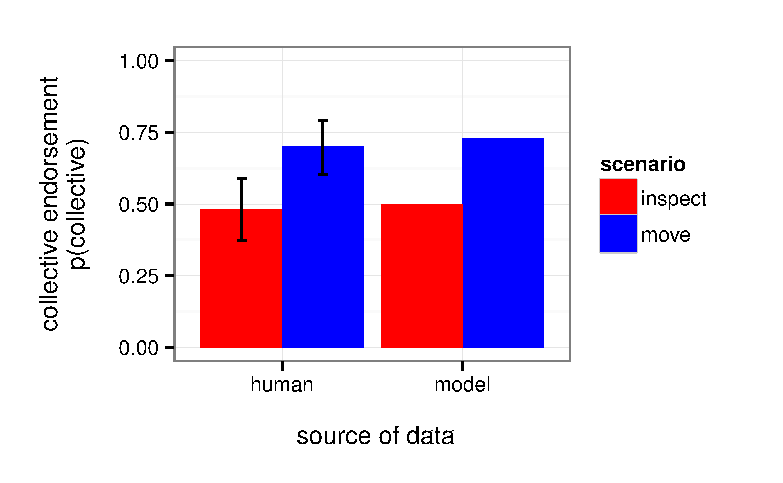
\includegraphics[width=.8\linewidth]{plots/heavymodel.eps}
	\vspace{0pt}
	\caption{Fitted model predictions and human data from Expt.~2 for collective interpretations of \emph{heavy}; variability of context (i.e., ``random'' vs.~``regular'') is modeled by noise in the collective interpretation, and the scenario manipulation (i.e., ``inspect'' vs.~``move'') is modeled by speaker's perceptual access to knowledge of the state (``full'' vs.~``partial'').} \label{heavymodel}
\end{figure}

Next, for \emph{big} and \emph{tall} we again predict collective endorsement, this time collapsing over the scenario manipulation. As with \emph{heavy}, we again fit predicate-specific values for collective interpretation noise. Also, we cheapen the cost of the ambiguous utterance relative to the unambiguous ones; in place of the flat prior distribution over possible utterances used above, here we set the prior such that \texttt{ambiguous} is twice as cheap as \texttt{collective} or \texttt{distributive}. With no other changes to model parameters, we generate the predictions plotting in Fig.~\ref{bigtallmodel}; once again, the fit is near perfect.

\begin{figure}[h]
	\centering
	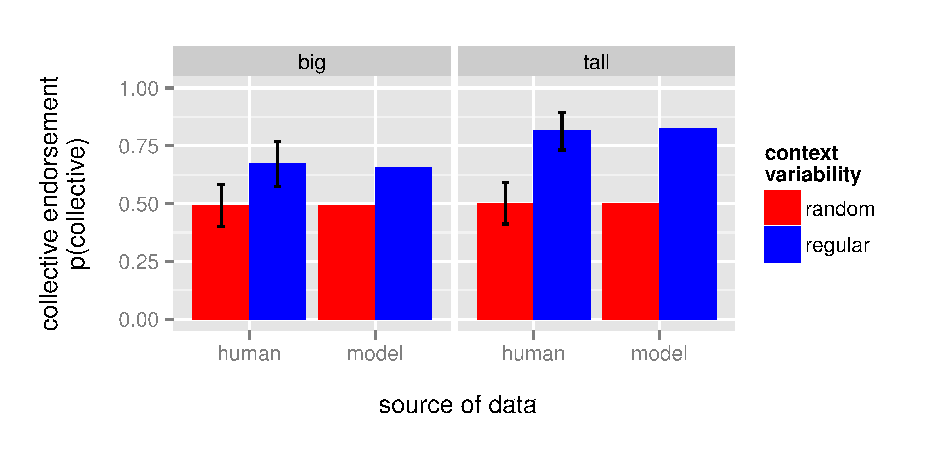
\includegraphics[width=.8\linewidth]{plots/bigtallmodel.eps}
	\vspace{0pt}
	\caption{Fitted model predictions and human data from Expt.~2 for collective interpretations of \emph{big} and \emph{tall}; variability of context (i.e., ``random'' vs.~``regular'') is modeled by noise of collective interpretation.} \label{bigtallmodel}
\end{figure}

In addition to the match between the qualitative predictions of our model and the human data from Expt.~2, we have shown that fitting predicate-specific parameters for noise and utterance cost yields near exact quantitative predictions of behavior. Put simply, our model of plural predication succeeds. Collective interpretations become more likely as the properties they name become more predictable in context.


\section{General discussion}

We began with an age-old observation about collective interpretations for gradable predicates with plural subjects: some predicates admit collective interpretations, while others strongly (or totally) resist them. This phenomenon, dubbed ``stubborn distributivity'' after those predicates that ostensibly refuse collective interpretations, has been documented and described, even characterized in terms of semantic constraints. But an explanation of the phenomenon has proven elusive. Here, we offer an explanation: stubbornly distributive predicates are so because the collective properties they name are unpredictable, or unstable, in context; this unpredictability results in a noisy collective interpretation, something speakers and listeners recognize as ineffective for communicating efficiently about their world.

We found evidence for this information-theoretic explanation over the course of two experiments. First, in Expt.~1, we verified the phenomenon of stubborn distributivity, demonstrating that \emph{big} resists collective interpretations while \emph{heavy} admits them. The results of experiment also demonstrate the role of speaker access to knowledge, something both speakers and listeners track as they communicate with each other. In a scenario where speakers plausibly lacked epistemic support for a distributive interpretation, collective interpretations became more likely.

In Expt.~2, we replicated the speaker knowledge effect while testing more directly the role of contextual predictability in collective predication. After manipulating the regularity of the predication context, we found that more regular contexta yielded greater rates of collective paraphrase endorsement for \emph{each} of the predicates tested. We thus confirmed our hypothesis: increasing contextual predictability of collective properties --- by increasing the regularity of the contexts themselves -- increases rates collective interpretations. In other words, rates of collective interpretation were shown to be determined by an interaction between the property named and the context of predication.

Having both demonstrated and quantified the role of contextual predictability and speaker knowledge in plural predication, we then formalized the role of each factor in a computational model of communication. Our model, conceived within the Rational Speech-Act framework, employed standard semantics to achieve not only accurate qualitative, but accurate quantitative predictions of our human data. Speaker knowledge affected collective interpretations by removing epistemic support and thereby decreasing a speaker's utility for distributive interpretations. Contextual predictability had a similar effect: noisier, less predictable collective interpretations are less effective at correctly communicating about the world; being less useful, they are less likely.

In what follows, we discuss in more detail the consequences of these findings for the theories they inform.

\subsection{Implications for semantic theories of plurality}

Plural predication is heavily dependent on the context in which that predication occurs. Taking as our starting point the null hypothesis that all such predications are potentially ambiguous between collective and distributive interpretations, we have seen that speakers and listeners track properties of the context (and of each other) as they endeavor to resolve this ambiguity. By considering plural predication within an articulated formal theory of communication (i.e., the Rational Speech-Act framework), we have identified and isolated two elements of this calculus: a) speaker's access to knowledge, and b) noise in the estimation of properties. For present purposes, it is this latter element, contextual predictability, that features most prominently in our explanation of stubborn distributivity.

Recall that current theories of the phenomenon describe it as a constraint on the sort of subjects certain predicates may compose with. Concretely, stubbornly distributive predicates refuse pluralities from their basic, un-starred denotations. To compose with a plural subject, the predicate must be closed under sum-formation. No such restriction applies to complaisantly collective predicates, which welcome pluralities in their un-starred denotations. The terrain of denotations in \Next results; note the absence of pluralities from the basic denotation of \texttt{big}.

\ex. \emph{Stubbornly distributive} \texttt{big}:
\a. \sem{\texttt{big}} = \{\texttt{a}, \texttt{b}, \ldots\}
\b. \sem{*\texttt{big}} = \{\texttt{a}, \texttt{b}, \texttt{a}$\oplus$\texttt{b}, \ldots\}

\ex. \emph{Complaisantly collective} \texttt{heavy}:
\a. \sem{\texttt{heavy}} = \{\texttt{a}, \texttt{b}, \texttt{a}$\oplus$\texttt{b}, \ldots\}
\b. \sem{*\texttt{heavy}} = \{\texttt{a}, \texttt{b}, \texttt{a}$\oplus$\texttt{b}, \ldots\}

Given the prohibition on plural subjects in their basic denotations, stubbornly distributive predicates simply cannot deliver collective interpretation, which result from direct predication between a singular, or basic predicate and a plural subject. At the very least, the results of our experiments demonstrate that stubborn distributivity should not (indeed, cannot) manifest in terms of an all-out prohibition against collective interpretations. Even unabashed stubbornly distributive predicates like \emph{big} yield greater rates of collective interpretations when context supports them. And it is the way that context supports collective interpretations that provides the key to understanding stubborn distributivity: contextual predictability.

Complaisantly collective predicates like \emph{heavy} or \emph{expensive} do not require support from context to ensure that their collective properties are predictable. The properties of collective weight and price are inherently stable in context; there exists but one way to evaluate these properties, and they persist despite changing physical arrangement. Not so for the collective properties named by stubbornly distributive predicates like \emph{big} or \emph{round}, which name properties of size or shape. Owing to uncertainty in evaluation strategy, compounded by definitional dependence on physical arrangement, these collective properties are relatively unpredictable, unstable, and as a result difficult for speakers and listeners to coordinate on in the absence of additional contextual or linguistic cues. Grammar might encode stubborn distributivity as a preference against plural arguments for certain predicates, but here we suggest a lower level explanation for this preference: stubbornly distributive predicates name collective properties that are difficult to accurately communicate. Increasing the contextual predictability of these properties as we did in Expt.~2 decreases this difficulty and thereby increases the likelihood of collective interpretations.

Further evidence for the non-trivial role of contextual predictability in collective predication comes from data demonstrating that one and the same predicate receives varying rates of collective interpretations depending on the noun that serves as its subject. In a pilot study of ambiguity resolution in naturally-occurring examples of plural predication, we identified the 40 most frequent subject-predicate combinations in a plural predication frame (i.e., \emph{The NOUNs were ADJECTIVE}) in the British National Corpus.\footnote{The sentences in \ref{bnc} were extracted from the British National Corpus Online service, managed by Oxford University Computing Services on behalf of the BNC Consortium. All rights in the texts cited are reserved.} Of those pairs, the predicate \emph{small} appeared four times, each with a different subject. Using the same paraphrase methodology from Expt.~2, we had 80 subjects rate distributive ``each'' vs.~collective ``together'' paraphrases of the four sentences in \Next.

\ex. \label{bnc}\a. The classes were small.
\b. The rooms were small.
\b. The children were small.
\b. The numbers were small.

\begin{figure}[h]
	\centering
	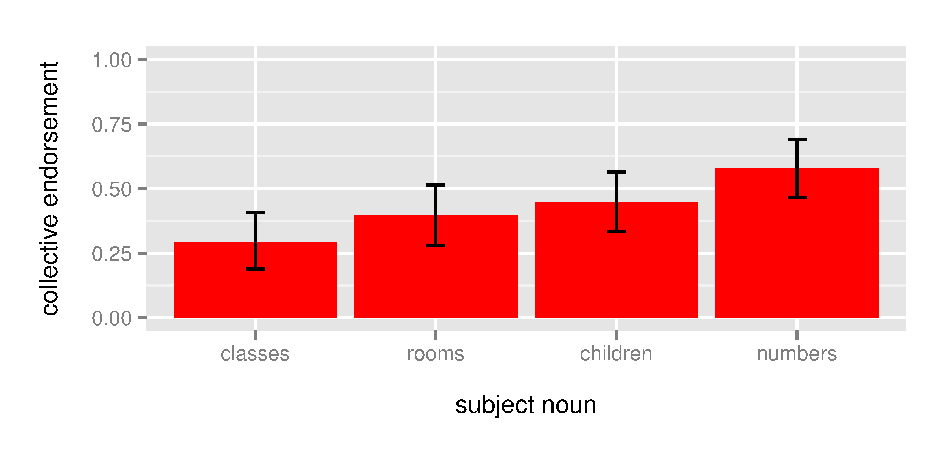
\includegraphics[width=.9\linewidth]{plots/small_coll_plot.eps}
	\vspace{0pt}
	\caption{Collective paraphrase endorsement rates for different nouns serving as the subject to the predicate \emph{small}.} \label{smallcoll}
\end{figure}

If stubborn distributivity were a binary, predicate-level phenomenon hard-coded into the semantics of these words, we should find no effect of the subject noun in the determination of their distributive vs.~collective interpretations: stubbornly distributive predicates, regardless of their subject, should always be maximally distributive. As Fig.~\ref{smallcoll} demonstrates, however, they are not. More importantly, the subject \emph{numbers} stands out in its relatively high rates of collective endorsement with the predicate \emph{small}.\footnote{A linear mixed effects model predicting collective endorsement rate by subject noun finds that sentences with the subject \emph{numbers} are receive greater rates of collective endorsement than do sentences with \emph{children} ($\beta=-0.15$, $SE=0.07$, $t=-2.24$, $p<0.05$), \emph{rooms} ($\beta=-0.19$, $SE=0.07$, $t=-2.73$, $p<0.01$), or \emph{classes} ($\beta=-0.27$, $SE=0.07$, $t=-3.87$, $p<0.01$).} Allow us to suggest an explanation for the exceptional behavior of \emph{numbers} in terms that by now ought to ring familiar: faced with the task of evaluating the relative size of a hypothetical set of numbers, participants converge on a single strategy, namely summing them up. In other words, the collective size of numbers is relatively predictable in context, more so than the collective size of children (determined by, e.g., height, weight, age, etc.) or of rooms and classes (determined by, e.g., number of occupants, seating capacity, overall volume, etc.). The same mechanism we saw at play in the context manipulation of Expt.~2 rears its head again here: contextual predictability of the collective property determines availability of collective interpretations.

Note that subject nouns already played a crucial role in the disambiguation of plural predications. We saw that physically aggregating a plurality using an atomizing noun like \emph{pile} or \emph{stack} greatly increases the availability of collective interpretations. Again, semantics might attend to the atomic status of the resulting noun phrase in its evaluation of stubborn distributivity (\emph{the pile of boxes} name a single atom, while \emph{the boxes} most likely does not), but pragmatics provides us with an explanation for why these nouns seem to unlock the collective interpretation. Just as our contextual manipulation in Expt.~2 increased contextual predictability of collective size or height by increasing the likelihood of encountering a plurality of boxes in a specific physical arrangement, so too do atomizing nouns. The arrangement of a \emph{stack} or \emph{pile} of boxes is much more regular across contexts than an abstract collection thereof. It is this regularity introduced by the atomizing noun that permits an otherwise elusive collective interpretation; the information-theoretic mechanism remains the same.

To understand this mechanism, namely how contextual predictability affects the calculus of interpretation choice, we modeled its contribution explicitly within a computational model of plural predication.


\subsection{Implications for formal models of pragmatics}


\section{Conclusion}


\appendix

\section{Full mixed effects linear regression models from Expt.~1}\label{expt1results}


Table \ref{expt1analysis1} presents model coefficients for the full mixed logistic regression model used in the analysis of disambiguating paraphrases in Expt.~1. The model predicts collective referent choice from fixed effects for disambiguating utterance and trial, as well as random by-participant, by-predicate, and by-scenario intercepts. The model also includes random slopes for participants grouped by utterance. The fixed effects predictors were centered before analysis.

\begin{table}[h!] 
	\centering \caption{Full logistic regression model from paraphrase analysis of Expt.~1.} \label{expt1analysis1}
\begin{tabular}{lrrrr}\toprule
	&	Coef $\beta$	&	SE($\beta$)	&	\multicolumn{1}{c}{ \textbf{z}}	&	\multicolumn{1}{c}{$p$}\\ \midrule
Intercept	&	-0.43	&	0.49	&	-0.88	&	0.38\\
Utterance	&	5.50	&	0.94	&	5.87	&	\textbf{$<$0.01}\\
Trial	&	0.07	&	0.08	&	0.81	&	0.42\\
\bottomrule
\end{tabular}
\end{table}

Table \ref{expt1analysis2} presents model coefficients for the full mixed logistic regression model used in the analysis of bare utterances in Expt.~1. The model predicts collective referent choice from fixed effects for predicate, scenario, and trial, as well as random by-participant intercepts and sloped grouped by trial. Fixed effects predictors were centered before analysis.


\begin{table}[h!] 
	\centering \caption{Full logistic regression model from bare utterance analysis of Expt.~1.} \label{expt1analysis2}
	\begin{tabular}{lrrrr}\toprule
		&	Coef $\beta$	&	SE($\beta$)	&	\multicolumn{1}{c}{ \textbf{z}}	&	\multicolumn{1}{c}{$p$}\\ \midrule
		Intercept	&	-4.65	&	1.49	&	-3.12	&	\textbf{$<$0.01}\\
		Pred-heavy	&	3.05	&	1.23	&	2.48	&	\textbf{$<$0.05}\\
		Pred-tall	&	3.63	&	1.29	&	2.82	&	\textbf{$<$0.01}\\
		Trial	&	-0.17	&	0.20	&	-0.84	&	0.40\\
		\bottomrule
	\end{tabular}
\end{table}
 


\section{Full mixed effects linear regression model from Expt.~2}\label{expt2results}

The following table presents model coefficients for the full mixed linear regression model used in the analysis of Expt.~2. The model predicts normalized collective endorsement ratings from fixed effects for context, predicate, scenario, and trial, as well as random by-participant intercepts and slopes grouped by trial. The fixed effects predictors were centered before analysis.

\begin{table}[h!] 
	\centering \caption{Full logistic regression model from analysis of Expt.~2.} \label{expt2analysis}
\begin{tabular}{lrrrr}\toprule
	&	Coef $\beta$	&	SE($\beta$)	&	\multicolumn{1}{c}{ \textbf{t}}	&	\multicolumn{1}{c}{$p$}\\ \midrule
Intercept	& 	0.58	&	0.03	&	17.08	&	\textbf{$<$0.01} \\
Pred-heavy	&	0.02	&   0.04	&	0.60	&	0.55 \\
Pred-tall	&	0.07	&	0.04	&	2.00	&	\textbf{$<$0.05}\\
Context		&	0.18	&	0.07	&	2.70	&	\textbf{$<$0.01}\\
Scenario	& 	0.00	&	0.07	& 	-0.02	&	0.98 \\
Trial		&	-0.01	&	0.02  	&	-0.36	&   0.72 \\
Pred-heavy:Context	&	-0.07	&	0.08	&	-0.98	&	0.33 \\
Pred-tall:Context	&	0.13	&	0.08	&	1.72	& \textbf{0.09} \\
Pred-heavy:Scenario	&	0.21	&	0.08	&	2.77	&	\textbf{$<$0.01} \\
Pred-tall:Scenario	&	0.07	&	0.08	&	0.95	& 0.35\\
\bottomrule
\end{tabular}
\end{table}


%\bibliographystyle{sp}
\bibliography{greg.bib}

\begin{addresses}
	\begin{address}
		Gregory Scontras \\
		Street1 \\
		City1 \ldots \\
		\email{author1@email}
	\end{address}
	\begin{address}
		Noah D.~Goodman \\
		Street2 \\
		City2 \dots \\
		\email{author2@email}
	\end{address}
	% repeat if needed.
\end{addresses}



\end{document}
